\documentclass[11pt,a4paper]{article}
\usepackage[utf8]{inputenc}
\usepackage[T1]{fontenc}
\usepackage{amsmath,amssymb,amsfonts,amsthm}
\usepackage{booktabs}
\usepackage{graphicx}
\usepackage{geometry}
\usepackage{hyperref}
\usepackage{xcolor}
\usepackage{caption}
\usepackage{setspace}
\onehalfspacing

\geometry{margin=0.85in}
\hypersetup{colorlinks=true,linkcolor=blue,citecolor=blue,urlcolor=blue}
\newtheorem{proposition}{Proposition}

\title{\textbf{Attention with a Calibrated Off Switch: Causal FIR Key Smoothing,\\ the Score-Shift Pathology, and Selective Silence in Rectified Attention (\texttt{pn\_fir\_tau})}}
\author{Maxim Zhukov\footnote{\href{https://orcid.org/0009-0005-9238-3778}{ORCID: 0009-0005-9238-3778}} \\ Independent Research \\ \small Reproducibility Package: \texttt{src/}, \texttt{experiments/exp1..6}, \\ \texttt{exp4b}, \texttt{exp4c}, \texttt{exp4e}, \texttt{exp4f}, \texttt{exp4g}, \texttt{exp4h}, \\ \texttt{results/}, \texttt{run\_all\_and\_build\_figures.py}}
\date{October 2026}

\begin{document}
\maketitle

\begin{abstract}
Softmax attention cannot say ``nothing found'': a simplex-constrained head must distribute $1.000$ units of context weight even when no key matches the query, and pre-trained models pay with attention sinks, massive outliers that degrade low-bit quantization \cite{bondarenko2023quantizable,zuhri2025softpick,sun2024massive}, and RAG-style hallucinations on unanswerable queries. The off-switch mechanism itself is established prior art: ReLA replaces Softmax with ReLU and its heads ``attend to nothing'' \cite{zhang2021rela}; Softpick scales rectified normalization to 340M--1.8B with a 0\% sink rate \cite{zuhri2025softpick}. The open question is the interaction layer audited here. A parameter-free 7-tap causal FIR low-pass filter ($\sigma=2.0$) applied strictly to the key stream $K$ lets one layer bind a queried key onto the adjacent value slot, lifting non-bijective single-layer associative recall from $44.5\% \pm 0.9\%$ to $100.0\% \pm 0.0\%$ and removing exact-decoy vulnerability on the legacy benchmark ($\Delta = 0.000$ at decoy noise $\epsilon \in \{0.05, 0.2, 0.5, 1.0\}$). The same smoothing shifts scores downward and starves rectification: fixed-$\tau{=}0$ power-norm falls to $64.4\% \pm 6.8\%$ with $91.3\% \pm 8.6\%$ negative scores and $44.5\% \pm 23.0\%$ dead rows; Softmax masks this shift (translation-invariant), rectification does not (Proposition~\ref{thm:dilemma}). One learnable threshold $\tau$ per layer (\texttt{pn\_fir\_tau}) restores $100.0\%$ recall and keeps unanswerable rows silent under pure cross-entropy ($\sum_{j} W_{t,j} = 0.002 \pm 0.002$ vs.\ $0.100 \pm 0.005$ for virtual sinks) reaches matched-precision WikiText-2 parity on 2,400 steps ($\le 0.3\%$ across five variants, single seed). We release fused Triton kernels (no $\exp()$, $O(N)$ attention VRAM) and a full measurement record, including an instrumented retraction of our initial end-to-end latency claim.


\end{abstract}

\section{Introduction: Practical Motivation and Related Work}

Why modify the core attention mechanism of a Transformer? In practical sequence modeling, standard scaled dot-product Softmax attention \cite{vaswani2017attention} forces practitioners to pay a steep architectural and computational tax for two basic operations: \textbf{(A) reading the value token that follows a matched key in context} (in-context learning and associative lookup), and \textbf{(B) doing nothing when a specialized attention head finds no relevant match in the context} (residual-stream preservation in RAG, tool use, and memory lookup).

\subsection{Practical Problem 1: Compressing Two-Layer Induction Heads into a Single Layer (\texttt{sm\_fir} / \texttt{pn\_fir\_tau})}

Associative retrieval---locating a context key $k^*$ that matches a query and routing the value $v^*$ stored at an adjacent position $j^*+1$ (\texttt{[... key A, value B ... query A] -> B})---is the foundational mechanism of in-context learning in Large Language Models (LLMs), enabling models to copy variable names, track entity attributes, and extract facts from prompts \cite{olsson2022induction}. In a standard Transformer, however, \textbf{a single token-level attention layer is structurally incapable of content-addressable key-value induction}: dot-product similarity $S_{t,j} = \langle Q_t, K_j \rangle / \sqrt{d_k}$ matches the query $Q_t$ (encoding $k^*$) against the key vector $K_{j^*}$ at the key slot $j^*$, whereas the target value token $v^*$ resides at the adjacent slot $j^*+1$, whose unfiltered key vector $K_{j^*+1} = W_K E(v^*)$ carries zero information about $k^*$ whenever keys and values are independently paired. As proved by Olsson et~al.\ \cite{olsson2022induction}, a standard Transformer must dedicate \textbf{at least two sequential layers} to solve this task: Layer~1 (\emph{previous-token head}) shifts token $j^*$ into the residual stream of position $j^*+1$, and only in Layer~2 (\emph{induction head}) can attention match $Q_t$ against the composite representation at $j^*+1$. In compact or edge Transformers (4--12 layers), spending early layers and residual-stream bandwidth just to shift adjacent tokens is an expensive waste of depth.

Applying a parameter-free causal Finite Impulse Response (FIR) low-pass filter strictly to the key stream $K$ along the sequence dimension (the convolutional ancestors of this move are RWKV's learnable 2-tap token shift \cite{peng2023rwkv} on the R/K/V streams and the searched depthwise convolutions of \emph{Primer} \cite{so2021primer}; ours is a fixed zero-parameter $K_f=7$ half-Gaussian low-pass strictly on $K$) blends the representation of $k^*$ at position $j^*$ forward into position $j^*+1$:
\begin{equation}
\label{eq:fir_blend}
\tilde{K}_{j^*+1} = h_0 K_{j^*+1} + h_1 K_{j^*} + \sum_{m=2}^{K_f-1} h_m K_{j^*+1-m}.
\end{equation}
By Eq.~\eqref{eq:fir_blend}, $\tilde{K}_{j^*+1}$ now contains a weighted component $h_1 K(k^*)$ while both the query $Q_t$ and the value stream $V_{j^*+1} = W_V E(v^*)$ remain unfiltered, so \textbf{a single attention head querying for $k^*$ can attend directly to the value slot $j^*+1$ and read out $v^*$}---lifting single-layer non-bijective recall from $44.5\%$ (\texttt{sm}) to $100.0\% \pm 0.0\%$ (\texttt{sm\_fir} and \texttt{pn\_fir\_tau}) at a latency cost of just $+1.5\%\text{--}2.0\%$ in \texttt{sm\_fir}.

\subsection{Practical Problem 2: Preventing RAG Context Hallucinations and Eliminating Attention-Sink Outliers (\texttt{pn\_fir\_tau})}

In a multi-layer Transformer, the residual stream acts as a shared communication bus ($y_t = x_t + \sum_{j \le t} W_{t,j} V_j$). Most specialized attention heads (e.g., heads looking up an entity attribute or an answer in a retrieved RAG passage) are only relevant on a small fraction of tokens; when a retrieved passage does not contain the queried fact (\textbf{unanswerable query}), the head \emph{should stay completely silent} ($\sum_{j \le t} W_{t,j} = 0$) so that the existing residual representation $x_t$ is preserved uncorrupted. Because standard Softmax enforces $\sum_{j=0}^{t} W_{t,j} \equiv 1$ for every query $t$, it causes two major practical failures (recently modelled as Softmax's two missing primitives, abstention and noise filtering \cite{wang2026abstention}): (1) \textbf{RAG context hallucinations on unanswerable queries}, where the head is forced to overwrite the residual state $x_t$ with a weighted average of irrelevant context values $V_j$; and (2) \textbf{Attention Sinks and quantization outliers} \cite{bondarenko2023quantizable}~\cite{xiao2024streamingllm}, where pre-trained LLMs turn the initial \texttt{BOS} token ($t=0$) into a ``trash bin'' by inflating its hidden activations into massive numerical outliers \cite{sun2024massive} ($W_V x_0 \approx 0$) that degrade INT8/INT4 post-training quantization \cite{bondarenko2023quantizable} (a failure mode rectified normalizers remove at 340M--1.8B scale with a low-bit win \cite{zuhri2025softpick}) and cause perplexity collapse in streaming KV caches whenever the initial sink tokens are evicted \cite{xiao2024streamingllm}.

In the sparse and quiet attention literature, two families have been proposed:
\begin{enumerate}
\item \textbf{Simplex-projected sparse normalizers (\texttt{Sparsemax} \cite{martins2016sparsemax}, $\alpha$-\texttt{Entmax} \cite{peters2019sparse}, \cite{correia2019adaptively}):} For $\alpha > 1$ and $p = \frac{1}{\alpha-1}$, $\alpha$-Entmax computes $W_{t,j}^{\text{entmax}}(s) = \max(s_j - \tau^*(s), 0)^p$, where $\tau^*(s)$ is the unique Lagrange multiplier solving $\sum_{j=0}^{t} \max(s_j - \tau^*(s), 0)^p = 1$. Because $\tau^*(s + c\mathbf{1}) = \tau^*(s) + c$, Sparsemax ($\alpha=2$) and Entmax ($\alpha=1.5, 1.1$) are translation-invariant, but because $\sum_{j=0}^{t} W_{t,j} \equiv 1$ everywhere, they \textbf{can never produce an all-zero row} (zero selective silence), and concentrating weight onto the single least-negative mismatching token actually \emph{increases} context hallucination rates ($32.4\%\text{--}34.4\%$ vs.\ $27.2\%$ for Softmax in Exp~5).
\item \textbf{Virtual-sink Softmax (\texttt{Softmax\_1} \cite{miller2023offbyone}, Quiet Softmax \cite{bondarenko2023quantizable}, Attention Sinks \cite{xiao2024streamingllm}):} Appending a virtual sink logit $\tau$ yields $W_{t,j} = \frac{\exp(s_j)}{\sum_{m=0}^t \exp(s_m) + \exp(\tau)}$, breaking shift-invariance so $\sum_{j=0}^t W_{t,j} < 1$, but retaining strictly positive exponential tails $\exp(s_j) > 0$ across all context positions ($\sum_j W_j = 0.100 \pm 0.005$ leakage on absent keys in Exp~5).
\item \textbf{Rectified (Sub-Simplex) Normalizers --- established prior art (ReLA \cite{zhang2021rela}, Softpick \cite{zuhri2025softpick}):} ReLA \cite{zhang2021rela} replaces Softmax with ReLU, observes sparsity without projection, reports heads that ``attend to nothing,'' and stabilises training via LayerNorm initialisation or gating; Softpick \cite{zuhri2025softpick} trains a rectified, deliberately non-sum-to-one normalizer at 340M--1.8B with a 0\% sink rate and better low-bit quantized accuracy than Softmax. \texttt{pn\_fir\_tau} differs from this line in one falsifiable respect: it couples a per-layer learnable threshold $\tau$ with a peak-driven silence gate, and the threshold exists to calibrate the score shift that causal key smoothing imposes --- not merely as a stability device.
\end{enumerate}

Given that map, the open problem addressed here is not whether attention can be silent --- prior art answers that --- but whether a rectified normalizer survives causal key smoothing. Our audit (Section~\ref{sec:limitations}) uncovers a striking paradox when training is dominated by positive retrieval examples: adding causal FIR on $K$ to Softmax (\texttt{sm\_fir}) lifts clean associative recall to $100.0\% \pm 0.0\%$, whereas adding the exact same causal FIR filter on $K$ to uncalibrated rectified power-normalization (\texttt{pn\_fir}, fixed $\tau=0$) degrades recall to $64.4\% \pm 6.8\%$ (Exp~1) and $88.8\% \pm 9.2\%$ (Exp~2), while row-mean centering (\texttt{pn\_fir\_c}) makes row mass dependent on within-row dispersion rather than absolute score level.

\paragraph{Scope.} This is a controlled mechanistic study of how causal FIR smoothing interacts with sub-simplex normalization; the 1.8M-parameter language model and the synthetic recall tasks are deliberately small sandboxes that isolate the mechanism, not evidence of LLM-scale behaviour. We frame the contribution as a calibrated diagnostic and tool, and treat scale-up as future work.

\section{Mathematical Formulation and Score-Shift Pathology}

Let $X \in \mathbb{R}^{B \times T \times D}$ be the input sequence with model dimension $D$, $H$ heads, and head dimension $d_k = D/H$. Linear projections $Q = X W_Q$, $K = X W_K$, and $V = X W_V$ have shape $\mathbb{R}^{B \times H \times T \times d_k}$.

\subsection{Causal FIR Low-Pass Filtering Strictly on the Key Stream $K$}

Non-causal FFT filtering (\texttt{sm\_fft}, \texttt{pn\_fft}, \texttt{qe\_pn\_fft}) multiplies the full-sequence spectrum by a Gaussian mask, which leaks future tokens into past keys ($\text{past\_key\_leak} = 0.785$). To guarantee strict autoregressive causality ($\text{past\_key\_leak} = 0.0$), we apply a causal depthwise 1D FIR filter of length $K_f = 7$ exclusively to the key stream $K$, with half-Gaussian weights using $\sigma = \max((K_f - 1)/3.0, 0.5) = (7 - 1)/3.0 = 2.0$ (\texttt{causal\_gaussian\_taps} in \texttt{src/pnfirtau\_attention.py}; Fig.~\ref{fig:17-schematic-fir-filter}):
\begin{equation}
\label{eq:fir_taps}
\begin{aligned}
h_m &= \frac{\exp\!\left(-\frac{1}{2}(m / \sigma)^2\right)}{\sum_{r=0}^{K_f-1} \exp\!\left(-\frac{1}{2}(r / \sigma)^2\right)}, \quad m \in \{0, \dots, 6\}, \\
h &= [0.3329,\; 0.2938,\; 0.2019,\; 0.1081,\; 0.0451,\; 0.0146,\; 0.0037].
\end{aligned}
\end{equation}
With causal left-padding of $K_f - 1 = 6$ zeros using the taps in Eq.~\eqref{eq:fir_taps}, $\tilde{K}_t = \sum_{m=0}^{\min(t, 6)} h_m K_{t-m}$ depends exclusively on indices $\le t$, while both $Q$ and $V$ remain unfiltered (Fig.~\ref{fig:15-schematic-architecture}), yielding scores $S_{t,j} = \langle Q_t, \tilde{K}_j \rangle / \sqrt{d_k}$ for $j \le t$.

\begin{figure}[ht!]
\centering
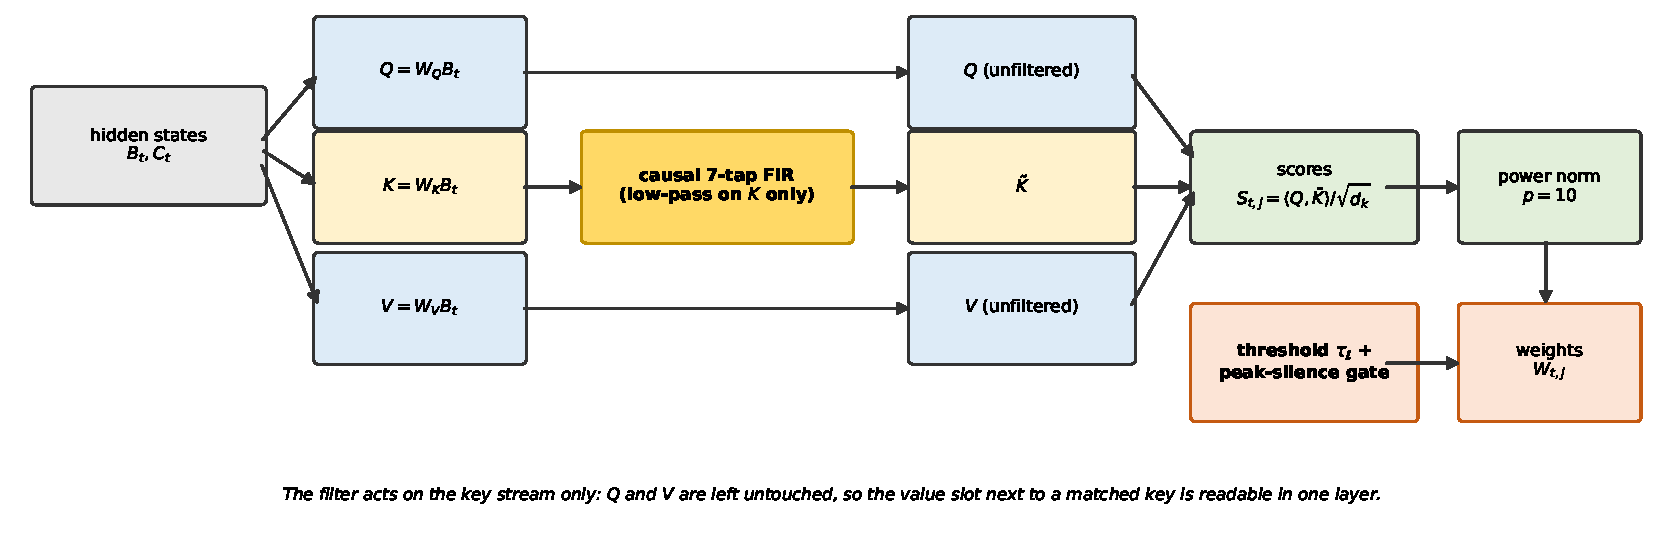
\includegraphics[width=0.98\textwidth]{figures/fig15_schematic_architecture.pdf}
\caption{Schematic of the rectified attention head architecture. The causal FIR low-pass filter acts on the key stream only; the query and value streams are left untouched, so a matched key can be read at the adjacent value slot within a single layer. Source: \texttt{paper\_en.tex} and \texttt{src/pnfirtau\_attention.py}.}
\label{fig:15-schematic-architecture}
\end{figure}

\begin{figure}[ht!]
\centering
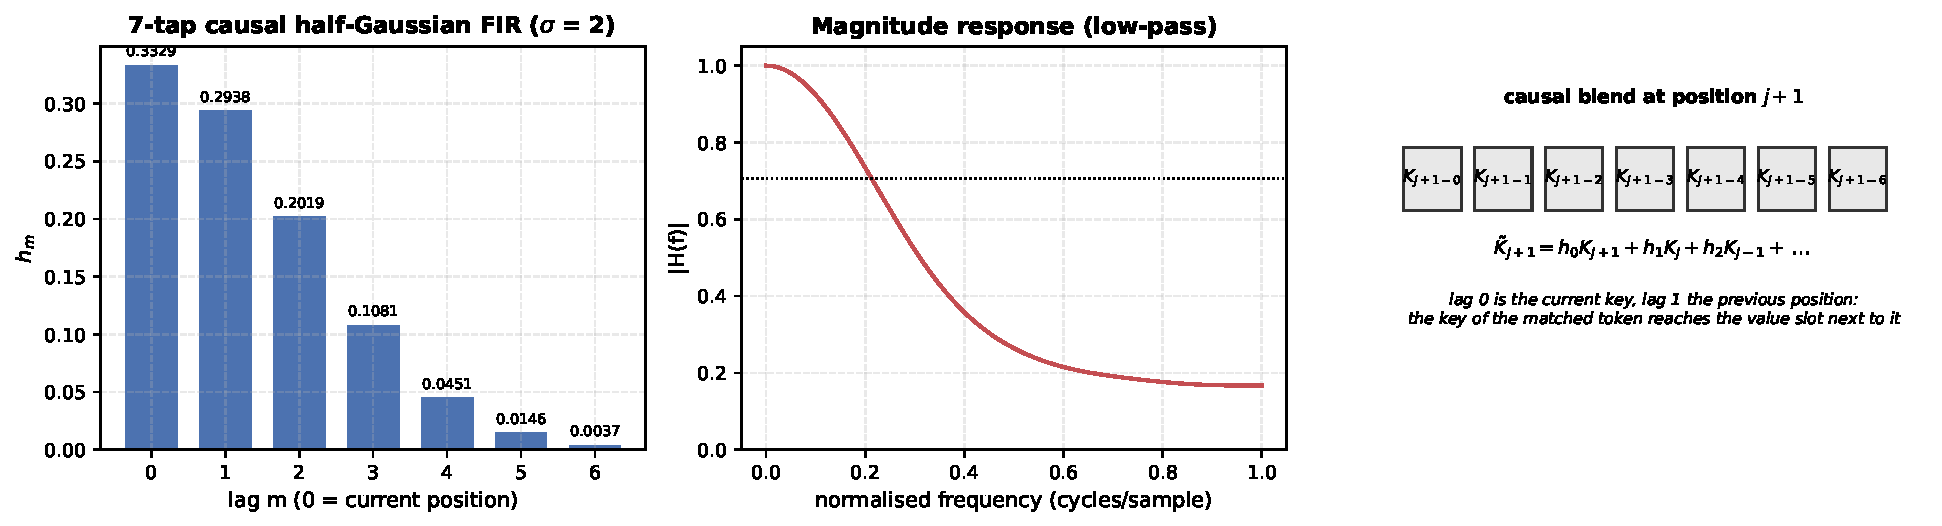
\includegraphics[width=0.98\textwidth]{figures/fig17_schematic_fir_filter.pdf}
\caption{Diagram of the 7-tap causal FIR low-pass filter. Left: the tap coefficients, computed by the production function \texttt{causal\_gaussian\_taps} and normalised to sum to one. Centre: the magnitude response of the same taps. Right: how the causal blend mixes the current key with the preceding positions. The computed taps coincide with the coefficients printed in the paper. Source: \texttt{src/pnfirtau\_attention.py} and \texttt{paper\_en.tex}.}
\label{fig:17-schematic-fir-filter}
\end{figure}



\subsection{Simplex vs.\ Sub-Simplex Normalizers, Shift-Ray Invariance, and Score-Shift Pathology}

\begin{proposition}[Mass Constancy Along Uniform Shift Rays]
\label{thm:dilemma}
Let $\Phi: \mathbb{R}^n \to [0, 1]^n$ be any attention row normalizer with total row mass $M(s) = \sum_{j=1}^n \Phi_j(s) \in [0, 1]$.
\begin{enumerate}
\item \textbf{(Simplex normalizers):} If $\Phi$ maps onto the probability simplex ($M(s) \equiv 1$ for all $s \in \mathbb{R}^n$, as in Softmax, Sparsemax, and $\alpha$-Entmax), then $M(s)$ is identically $1$ everywhere and selective silence ($M(s) \to 0$) is impossible on any score vector $s \in \mathbb{R}^n$.
\item \textbf{(Shift-invariant normalizers along uniform shift rays):} If $\Phi$ is translation-invariant ($\Phi(s + c\mathbf{1}) = \Phi(s)$ for all $s \in \mathbb{R}^n, c \in \mathbb{R}$), then its total row mass is constant along every uniform shift ray $\{s - c\mathbf{1} : c \in \mathbb{R}\}$, i.e., $M(s - c\mathbf{1}) = M(s)$ for all $c \in \mathbb{R}$. Consequently, $\Phi$ cannot transition from active retrieval ($M(s) \approx 1$) to selective silence ($M(s - c\mathbf{1}) \to 0$ as $c \to +\infty$) when all scores in a row are shifted downward by a common offset $c$.
\end{enumerate}
\end{proposition}

\paragraph{Why distinguish uniform shift rays from within-row dispersion (\texttt{pn\_fir\_c})?} Proposition~\ref{thm:dilemma}(2) characterizes behavior along \emph{uniform shift rays} $s \mapsto s - c\mathbf{1}$ (where within-row differences $s_j - s_m$ are preserved). A translation-invariant sub-simplex normalizer is not required to have constant mass across \emph{all} $s \in \mathbb{R}^n$: in row-mean-centered power-normalization (\texttt{pn\_fir\_c}, $S'_{t,j} = S_{t,j} - \mu_t$ with peak gate $g_t = \frac{\max_j (S_{t,j} - \mu_t)_+}{\max_j (S_{t,j} - \mu_t)_+ + \gamma}$), $M(S_t) = g_t$ is invariant to uniform shifts $S_t \mapsto S_t - c\mathbf{1}$ because $\max_j S_{t,j} - \mu_t$ is shift-invariant, yet $M(S_t)$ depends on the \textbf{within-row score dispersion} $\max_j S_{t,j} - \mu_t$ (and thus on query norm $\|Q_t\|_2$). This explains all three empirical regimes of \texttt{pn\_fir\_c}: (a) without a peak gate ($\gamma = \text{None}$, Exp~2 Table~\ref{tab:exp2}), subtracting $\mu_t$ guarantees $\max_j(S_{t,j} - \mu_t) > 0$ on every non-constant row, forcing $\sum_j W_{t,j} \equiv 1.000$; (b) on uncalibrated noise rows in positive-only training ($\gamma = 0.5$, Exp~1 Table~\ref{tab:exp1} and Exp~3 Table~\ref{tab:exp3}), random dot-product variance keeps $\max_j S_{t,j} - \mu_t \gg \gamma$, yielding $\sum W_{\text{noise}} = 0.938 \pm 0.007$ ($\text{gap} \le +0.021$); and (c) when trained end-to-end with 50\% unanswerable queries under Cross-Entropy loss ($\gamma = 0.5$, Exp~5 Table~\ref{tab:exp5}), \texttt{pn\_fir\_c} shrinks $\|Q_t\|_2$ on unanswerable queries to achieve partial silence ($\sum W_{\text{unans}} = 0.265 \pm 0.045$, $\text{gap} = +0.451 \pm 0.032$), but because $\max_j(S_{t,j} - \mu_t) > 0$ still holds on every non-constant row, it leaks $\approx 124\times$ more residual noise than \texttt{pn\_fir\_tau} ($0.002 \pm 0.002$) while degrading answerable override accuracy ($88.5\% \pm 8.9\%$ vs.\ $99.0\% \pm 0.7\%$).

Because $\|h\|_2^2 = \sum_{m=0}^{6} h_m^2 = 0.2518 < 1$ and each filtered key $\tilde{K}_j$ averages up to 7 adjacent tokens (most of which are negatively aligned filler tokens during positive-only training), the distribution of causal dot-product scores $S_{t,j} = \langle Q_t, \tilde{K}_j \rangle / \sqrt{d_k}$ contracts in variance and shifts negatively (Fig.~\ref{fig:16-schematic-score-shift-mechanism}):
\begin{itemize}
\item\sloppy \textbf{Softmax (\texttt{sm\_fir}), Sparsemax, and Entmax are translation-invariant:} Since $\operatorname{softmax}(S_t - c) = \operatorname{softmax}(S_t)$, Softmax is unaffected by negative offsets. In Exp~1, $100.0\%$ of query rows in trained \texttt{sm\_fir} have strictly negative scores ($\text{raw\_frac\_pos} = 0.0\%$, $\text{raw\_rows\_all\_neg} = 100.0\%$), yet \texttt{sm\_fir} achieves $100.0\% \pm 0.0\%$ accuracy.
\item \textbf{Rectified power-norm (\texttt{pn\_fir}) suffers dead-row starvation under positive-only training:} Uncalibrated power-norm rectifies scores at zero, $S^+_{t,j} = \max(S_{t,j}, 0)$. When $\max_{j \le t} S_{t,j} \le 0$, the entire row is clipped to zero, yielding $\hat{w}_{t,j} = 0$ and exact zero gradients ($\partial \mathcal{L} / \partial S_{t,j} = 0$). In Exp~1, $91.3\% \pm 8.6\%$ of raw scores in \texttt{pn\_fir} are negative and $44.5\% \pm 23.0\%$ of query rows are completely dead ($\text{raw\_rows\_all\_neg} = 44.5\% \pm 23.0\%$ across seeds).
\item \textbf{Row-mean centering (\texttt{pn\_fir\_c}) trades absolute level for within-row dispersion:} Subtracting the causal row mean $\mu_t = \frac{1}{t+1}\sum_{m=0}^{t} S_{t,m}$ forces roughly half of every noise row ($44.4\%$ of entries in Exp~1) above zero, driving noise attention mass to $\sum_j W_j = 0.938 \pm 0.007$ (Exp~1) and $1.000 \pm 0.000$ (Exp~2).
\end{itemize}

\begin{figure}[ht!]
\centering
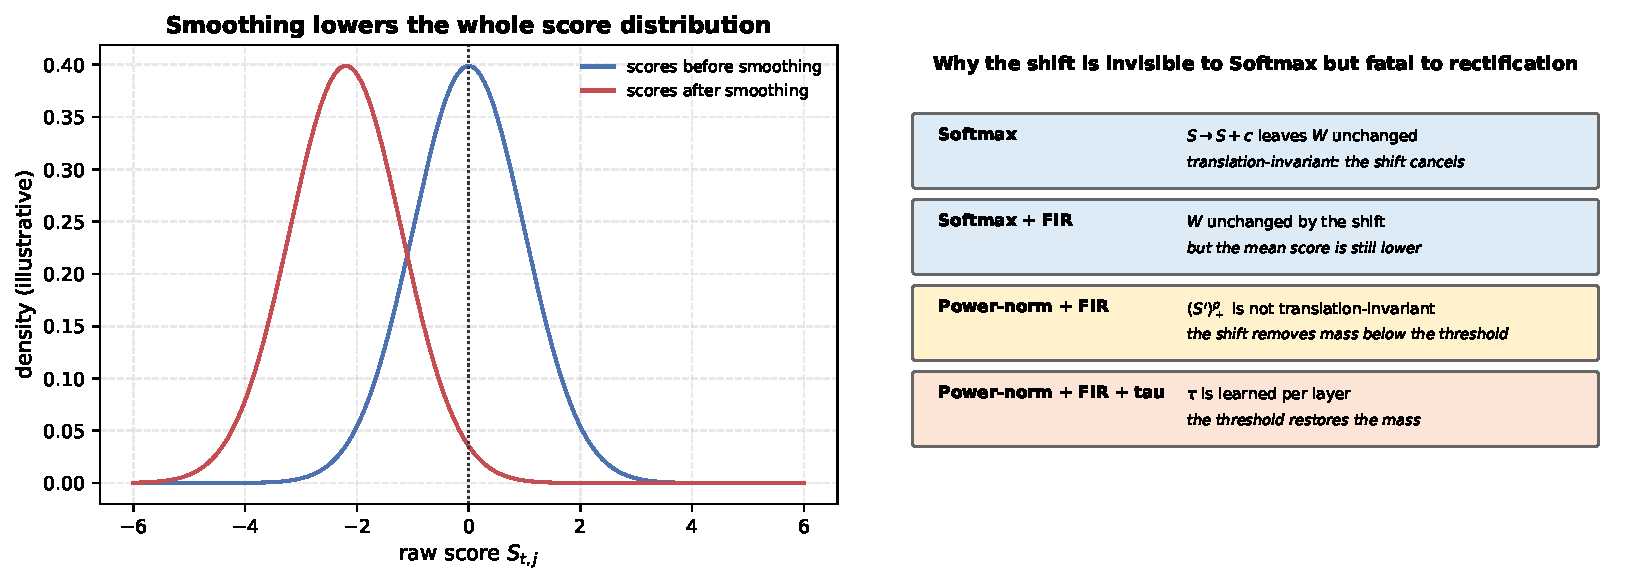
\includegraphics[width=0.98\textwidth]{figures/fig16_schematic_score_shift_mechanism.pdf}
\caption{Diagram of the score-shift pathology. Left: smoothing lowers the whole score distribution, which a translation-invariant normaliser cancels but a rectified one does not. Right: the four regimes and why a negative shift is invisible to Softmax yet removes mass under a fixed threshold. The left panel is a schematic illustration of the mechanism; the measured shift is quantified in the text and in the width-ladder figure. Source: \texttt{paper\_en.tex} (Proposition~1) and \texttt{src/pnfirtau\_attention.py}.}
\label{fig:16-schematic-score-shift-mechanism}
\end{figure}



\subsection{The \texttt{pn\_fir\_tau} Formulation and IO-Aware Fused Triton Kernels}

To calibrate the global score distribution without restoring within-row shift-invariance, \texttt{pn\_fir\_tau} introduces a single learnable scalar threshold $\tau \in \mathbb{R}$ per attention layer ($\tau_0 = 0.0$):
\begin{align}
\label{eq:pnfirtau}
S'_{t,j} &= (S_{t,j} - \tau)\cdot\mathbb{I}(j \le t), \qquad S^+_{t,j} = \max(S'_{t,j}, 0), \\
\label{eq:pn_weights}
\hat{w}_{t,j} &= \frac{(S^+_{t,j})^p}{\sum_{m=0}^{t} (S^+_{t,m})^p + \varepsilon}, \qquad g_t = \frac{\max_{0 \le m \le t} S^+_{t,m}}{\max_{0 \le m \le t} S^+_{t,m} + \gamma}, \qquad W_{t,j} = g_t \cdot \hat{w}_{t,j},
\end{align}
where $p = 10.0$, $\varepsilon = 10^{-12}$, and $\gamma = 0.5$ is the peak silence gate constant in Eqs.~\eqref{eq:pnfirtau}--\eqref{eq:pn_weights}. The total row weight is $\sum_{j=0}^{t} W_{t,j} = g_t \in [0, 1)$.

In eager PyTorch (\texttt{PnFirTauMHA}), evaluating Eqs.~\eqref{eq:pnfirtau}--\eqref{eq:pn_weights} materializes four $[B, H, N, N]$ intermediate tensors in HBM. In \texttt{src/triton\_pnfirtau.py}, we eliminate this bottleneck via three custom Triton \cite{dao2022flashattention} kernel suites: (1) \texttt{triton\_causal\_fir} (zero-copy strided $K_f=7$ causal FIR on $K$); (2) \texttt{PnFirTauTritonMHA} (\texttt{triton\_pn\_fir\_tau\_scores}, a single row-fused kernel replacing the 6-op eager score-to-weight chain); and (3) \texttt{PnFirTauFlashMHA} (\texttt{flash\_pn\_fir\_tau\_attention}, an online-tiled $O(N)$-VRAM FlashAttention-2 style kernel with uniform tile size $B_M = B_N = 64$). Crucially, once fused in SRAM registers, $(S'_{t,j})_+^{10}$ is evaluated in 3 register multiplications ($u^2, u^4, u^8 \cdot u^2$) with \textbf{zero transcendental \texttt{exp()} calls}, accumulates across tiles without online max-rescaling, computes exact analytical gradients in a single KV-parallel backward pass using the identity $D_t \triangleq \sum_{j=0}^t dW_{t,j}\hat{w}_{t,j} = \langle dO_t, O_t \rangle / g_t$ with deterministic per-block \texttt{FP64} reduction for $\partial\mathcal{L}/\partial\tau$, and includes early-exit tile branches when $\max u_{t,j} \le 0$ across a $64 \times 64$ tile (evaluated in Table~\ref{tab:exp4_skip}).

\section{Experimental Results and Algorithmic Audit}

The experiments below are presented in dependency order, not numerical order: $1 \to 2 \to 6 \to 4f/4g \to 3 \to 5 \to 4$.

\subsection{Experiment 1: Legacy 13-Stack Benchmark and Shortcut Audit}

Table~\ref{tab:exp1} reports the 3-seed evaluation (\texttt{1234, 2025, 3141}) of all 13 canonical stacks and 4 un-gated ($\gamma=\text{None}$) ablations on the legacy synthetic task ($V=24, D=32, T=15$, 2,000 epochs, where $\text{KEY} \in \{1..5\}$ is at $t=0$, $\text{VAL} = \text{KEY}+5 \in \{6..10\}$ is at $t=1$, filler $\in \{1..23\}$ is at $2..13$, and $\text{QUERY}=\text{KEY}$ is at $t=14$).

\begin{table}[ht!]
\centering
\caption{Experiment 1: Full 13-stack legacy benchmark and 4 un-gated ablations (3 seeds: \texttt{1234, 2025, 3141}, mean $\pm$ std). $W_{t,0}$ and $W_{t,1}$ denote query attention weight on the key slot ($t=0$) vs.\ value slot ($t=1$). Filter labels omit the default peak gate ($\gamma=0.5$); the last four rows use $\gamma=\text{None}$. Source: \texttt{results/exp1\_legacy\_13stacks.json}.}
\label{tab:exp1}
\scriptsize
\setlength{\tabcolsep}{0.8pt}
\begin{tabular}{llccccccccccc}
\toprule
Stack & Filter & Clean (\%) & KR (\%) & d@0.05 & d@0.5 & d@1.0 & nd1/8 (\%) & $\sum W_m$ & $\sum W_n$ & Gap & $W_{t,0}$ & $W_{t,1}$ \\
\midrule
\texttt{sm} & None & $71.5 \pm 1.4$ & $45.1$ & $91.7$ & $89.1$ & $86.8$ & $91.4/100.0$ & $1.000$ & $1.000$ & $+0.000$ & $0.130$ & $0.136$ \\
\texttt{sm\_fft} & FFT (Non-Causal) & $99.0 \pm 0.1$ & $49.8$ & $99.1$ & $99.2$ & $99.2$ & $99.1/99.8$ & $1.000$ & $1.000$ & $+0.000$ & $0.219$ & $0.068$ \\
\texttt{sm\_fir} & FIR-7 & $\mathbf{100.0 \pm 0.0}$ & $21.9$ & $100.0$ & $100.0$ & $100.0$ & $100.0/100.0$ & $1.000$ & $1.000$ & $+0.000$ & $0.984$ & $0.013$ \\
\texttt{pn} & None & $50.6 \pm 3.9$ & $43.2$ & $57.9$ & $55.6$ & $53.0$ & $57.2/74.6$ & $0.973$ & $0.955$ & $+0.001$ & $0.074$ & $0.227$ \\
\texttt{pn\_c} & Center & $58.1 \pm 8.6$ & $38.2$ & $72.3$ & $68.1$ & $63.3$ & $71.6/77.3$ & $0.993$ & $0.988$ & $+0.000$ & $0.119$ & $0.119$ \\
\texttt{pn\_tau} & $\tau$ & $55.9 \pm 9.7$ & $42.7$ & $66.7$ & $64.9$ & $62.0$ & $66.1/80.1$ & $0.848$ & $0.811$ & $+0.002$ & $0.085$ & $0.154$ \\
\texttt{pn\_fft} & FFT (Non-Causal) & $98.9 \pm 0.3$ & $48.7$ & $99.0$ & $99.0$ & $99.0$ & $99.0/99.4$ & $0.995$ & $0.995$ & $+0.000$ & $0.222$ & $0.075$ \\
\texttt{pn\_fft\_c} & FFT+C & $81.6 \pm 9.3$ & $20.9$ & $80.8$ & $80.9$ & $80.6$ & $80.8/83.2$ & $0.952$ & $0.952$ & $+0.002$ & $0.256$ & $0.028$ \\
\texttt{pn\_fir} & FIR & $64.4 \pm 6.8$ & $20.5$ & $65.5$ & $64.9$ & $64.7$ & $65.3/69.1$ & $0.512$ & $0.000$ & $+0.375$ & $0.389$ & $0.001$ \\
\texttt{pn\_fir\_c} & FIR+C & $\mathbf{100.0 \pm 0.0}$ & $22.3$ & $100.0$ & $100.0$ & $100.0$ & $100.0/100.0$ & $0.944$ & $0.938$ & $+0.017$ & $0.904$ & $0.037$ \\
\textbf{\texttt{pn\_fir\_tau}} & \textbf{FIR+$\tau$} & $\mathbf{100.0 \pm 0.0}$ & $20.6$ & $\mathbf{100.0}$ & $\mathbf{100.0}$ & $\mathbf{100.0}$ & $\mathbf{100.0/100.0}$ & $0.570$ & $0.375$ & $+0.191$ & $0.554$ & $0.012$ \\
\texttt{qe\_pn} & QE+PN & $71.2 \pm 1.1$ & $45.2$ & $91.5$ & $87.8$ & $83.8$ & $90.8/100.0$ & $0.941$ & $0.915$ & $+0.000$ & $0.136$ & $0.140$ \\
\texttt{qe\_pn\_fft} & QE+PN+FFT & $99.6 \pm 0.0$ & $41.4$ & $99.7$ & $99.7$ & $99.7$ & $99.7/99.0$ & $0.913$ & $0.907$ & $+0.003$ & $0.243$ & $0.074$ \\
\midrule
\texttt{pn\_ungated} & None ($\gamma{=}\text{None}$) & $49.7 \pm 4.1$ & $35.5$ & $62.9$ & $58.1$ & $53.7$ & $61.8/78.1$ & $0.999$ & $0.992$ & $+0.001$ & $0.136$ & $0.152$ \\
\texttt{pn\_fir\_ungated} & FIR ($\gamma{=}\text{None}$) & $71.7 \pm 19.5$ & $21.3$ & $71.8$ & $71.7$ & $71.8$ & $71.8/72.5$ & $0.564$ & $0.000$ & $+0.517$ & $0.414$ & $0.092$ \\
\texttt{pn\_fir\_c\_ungated} & FIR+C ($\gamma{=}\text{None}$) & $100.0 \pm 0.0$ & $18.7$ & $100.0$ & $100.0$ & $100.0$ & $100.0/100.0$ & $1.000$ & $1.000$ & $+0.000$ & $0.998$ & $0.002$ \\
\texttt{pn\_fir\_tau\_ungated} & FIR+$\tau$ ($\gamma{=}\text{None}$) & $100.0 \pm 0.0$ & $18.7$ & $100.0$ & $100.0$ & $99.9$ & $100.0/100.0$ & $1.000$ & $0.717$ & $+0.282$ & $0.999$ & $0.001$ \\
\bottomrule
\end{tabular}
\end{table}

\paragraph{Audit of Exp 1 Shortcuts.} Inspection of $W_{t,0}$ vs.\ $W_{t,1}$ in Table~\ref{tab:exp1} exposes two shortcuts in the legacy task: (1) because $\text{VAL} = \text{KEY}+5$ is a fixed bijection and $\text{KEY}$ is always at $t=0$, left-padded causal FIR acts as a boundary detector for $t=0$ ($W_{t,0}=0.984$ for \texttt{sm\_fir}, $0.554$ of $0.570$ for \texttt{pn\_fir\_tau}), predicting $\text{VAL}$ directly from $V_0 = W_V E(\text{KEY})$ without reading $t=1$; and (2) because clean filler at $2..13$ draws from $\{1..23\}$ (which includes competing keys $\{1..5\}$), injecting $n_d=8$ copies of $E(\text{KEY})$ overwrites competing keys with copies of the true key, explaining why \texttt{sm} rises from $71.5\%$ (clean) to $100.0\%$ ($n_d=8$).

\subsection{Experiment 2: True Content-Addressable Non-Bijective Recall \& Distractor Decoys}

To eliminate both shortcuts, Experiment~2 places $M=3$ randomly paired $(k_m, v_m)$ pairs ($k_m \in \{1..8\}$, independently permuted $v_m \in \{9..16\}$) at random non-overlapping interior positions $j_m \in [2, 38]$ in $T=48$, with filler strictly from $\{17..23\}$. True distractor decoys overwrite $n_d \in \{1,2,4,8\}$ isolated filler slots with $(1-\epsilon)E(k^*) + \epsilon E(\text{filler})$. We also evaluate \texttt{pn\_fir\_tau\_reg}, which adds a post-warmup (epoch $\ge 1000$) silence penalty $\lambda_{\text{sil}} = 0.05$ on auxiliary absent-key queries.

\begin{table}[ht!]
\centering
\caption{Experiment 2: True Content-Addressable Non-Bijective Associative Recall ($M=3$ pairs in $T=48$, 3 seeds: \texttt{1234, 2025, 3141}, mean $\pm$ std). Here $W_{t, j^*}$ and $W_{t, j^*+1}$ measure attention on the interior target key slot vs.\ target value slot. Source: \texttt{results/exp2\_content\_addressable\_decoy.json}.}
\label{tab:exp2}
\scriptsize
\setlength{\tabcolsep}{1.6pt}
\begin{tabular}{lccccccccccc}
\toprule
Model & Clean (\%) & $\epsilon{=}0.05$ & $\epsilon{=}0.2$ & $\epsilon{=}0.5$ & $\epsilon{=}1.0$ & nd1/2/4/8 & $W_{t, j^*}$ & $W_{t, j^*+1}$ & $\sum W_m$ & $\sum W_n$ & Gap \\
\midrule
\texttt{sm} & $44.5 \pm 0.9$ & $47.6$ & $44.5$ & $43.8$ & $46.5$ & $45.5 / 45.7 / 44.6 / 46.8$ & $0.035$ & $0.234$ & $1.000$ & $1.000$ & $+0.000 \pm 0.000$ \\
\texttt{pn} & $35.8 \pm 1.0$ & $35.9$ & $35.4$ & $34.4$ & $35.1$ & $35.1 / 36.6 / 36.1 / 35.8$ & $0.015$ & $0.237$ & $1.000$ & $1.000$ & $+0.000 \pm 0.000$ \\
\texttt{sm\_fir} & $\mathbf{100.0 \pm 0.0}$ & $\mathbf{95.9}$ & $\mathbf{95.9}$ & $95.2$ & $92.0$ & $95.1 / 89.9 / 77.7 / 56.2$ & $0.132$ & $\mathbf{0.792}$ & $1.000$ & $1.000$ & $+0.000 \pm 0.000$ \\
\texttt{pn\_fir} & $88.8 \pm 9.2$ & $85.9$ & $85.5$ & $84.7$ & $82.1$ & $84.1 / 80.0 / 71.0 / 61.2$ & $0.032$ & $0.830$ & $1.000$ & $0.261$ & $+0.739 \pm 0.117$ \\
\texttt{pn\_fir\_c} & $96.5 \pm 4.9$ & $93.7$ & $93.4$ & $92.8$ & $90.1$ & $92.5 / 88.9 / 78.2 / 63.2$ & $0.044$ & $0.866$ & $1.000$ & $1.000$ & $+0.000 \pm 0.000$ \\
\textbf{\texttt{pn\_fir\_tau}} & $\mathbf{100.0 \pm 0.0}$ & $95.5$ & $\mathbf{95.8}$ & $\mathbf{95.5}$ & $\mathbf{93.1}$ & $\mathbf{95.6 / 90.5 / 74.7 / 56.9}$ & $0.063$ & $\mathbf{0.729}$ & $0.826$ & $0.218$ & $+0.608 \pm 0.135$ \\
\textbf{\texttt{pn\_fir\_tau\_reg}} & $\mathbf{100.0 \pm 0.0}$ & $93.8$ & $93.1$ & $91.8$ & $87.4$ & $93.1 / 82.6 / 60.6 / 38.8$ & $0.034$ & $\mathbf{0.647}$ & $0.684$ & $\mathbf{0.000}$ & $\mathbf{+0.684 \pm 0.030}$ \\
\bottomrule
\end{tabular}
\end{table}

Table~\ref{tab:exp2} and Figures~\ref{fig:decoy}--\ref{fig:pathology} confirm that when the bijection and boundary shortcuts are removed: (1) unfiltered \texttt{sm} ($44.5\%$) and \texttt{pn} ($35.8\%$) fail; (2) causal FIR on $K$ physically binds $h_1 K(k^*)$ onto the value slot $j^*+1$, shifting attention directly to $j^*+1$ ($W_{t, j^*+1} = 0.792$ for \texttt{sm\_fir}, $0.729$ for \texttt{pn\_fir\_tau}, $0.647$ for \texttt{pn\_fir\_tau\_reg}); and (3) \texttt{pn\_fir\_tau\_reg} learns $\tau = +0.115 \pm 0.021$, driving both noise and absent-key attention mass to $0.000 \pm 0.000$ across all seeds ($\text{gap} = +0.684 \pm 0.030$).

\begin{figure}[ht!]
\centering
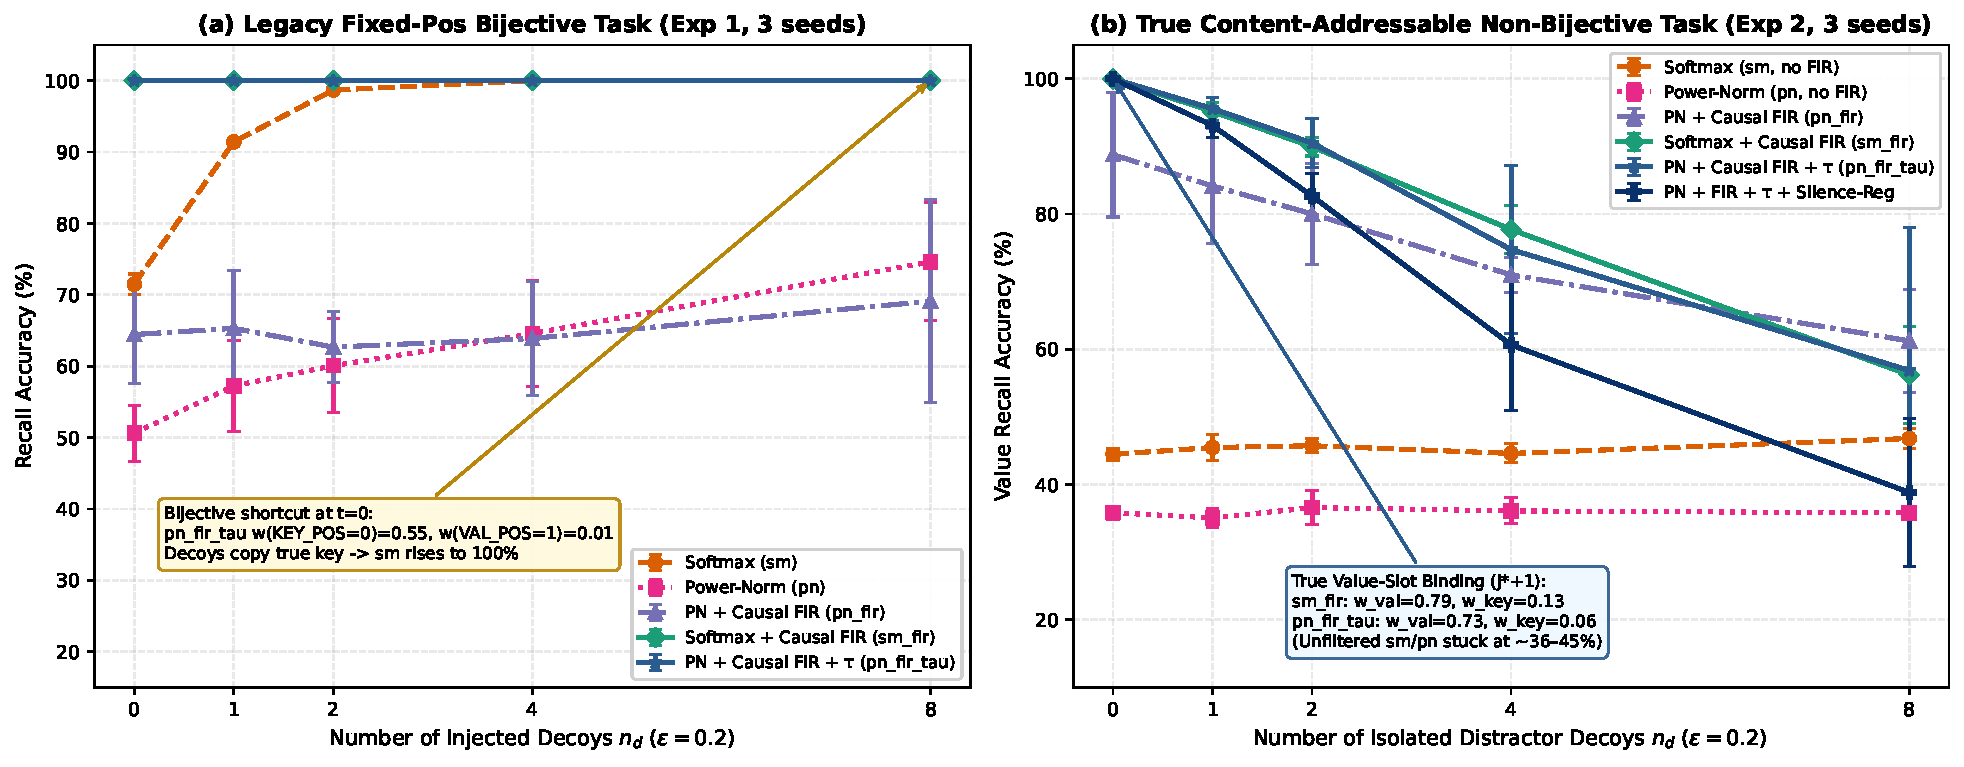
\includegraphics[width=0.98\textwidth]{figures/fig1_decoy_and_multidecoy.pdf}
\caption{Multi-decoy scaling ($n_d \in \{0,1,2,4,8\}$) and attention slot routing on the legacy fixed-position task (Exp~1, left) vs.\ the true content-addressable non-bijective task (Exp~2, right). Source: \texttt{results/exp1\_legacy\_13stacks.json} and \texttt{results/exp2\_content\_addressable\_decoy.json}.}
\label{fig:decoy}
\end{figure}

\begin{figure}[ht!]
\centering
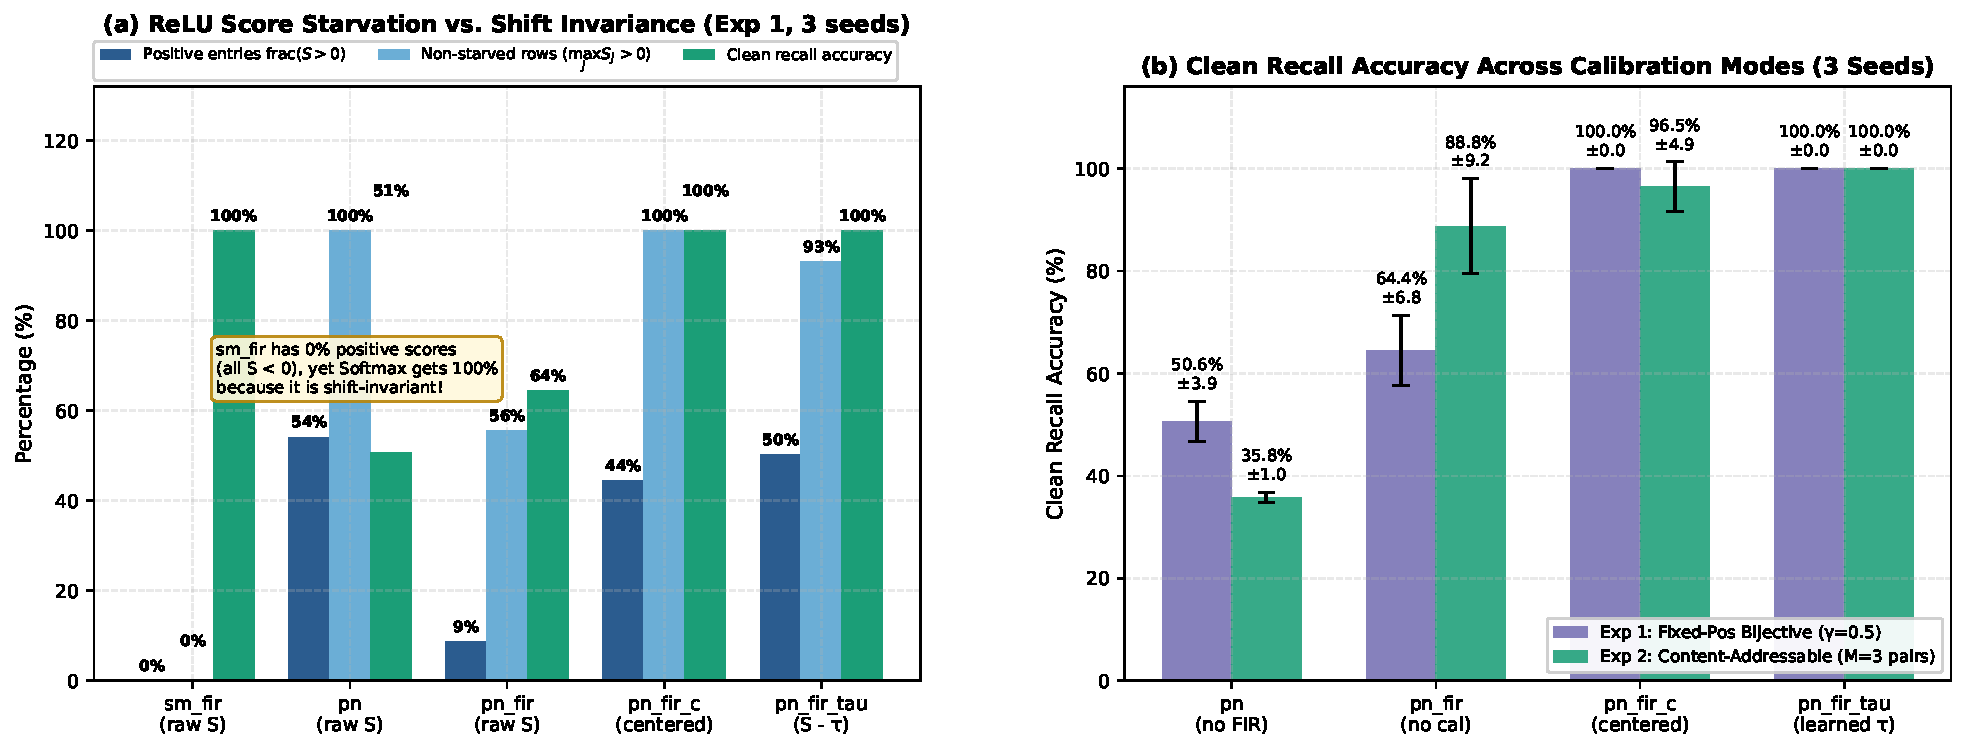
\includegraphics[width=0.98\textwidth]{figures/fig2_score_shift_pathology.pdf}
\caption{Pre-activation score-shift pathology in Exp~1 (left) and 3-seed clean recall accuracy across calibration modes in Exp~1 and Exp~2 (right). Source: \texttt{results/exp1\_legacy\_13stacks.json} and \texttt{results/exp2\_content\_addressable\_decoy.json}.}
\label{fig:pathology}
\end{figure}

\subsection{Experiment 6: Token-Shift Ablation (How Much Memory Does Robustness Need)?}

Exp~2's flooding result raises a precise follow-up: is the 7-tap low-pass doing work a 2-tap RWKV-style token shift cannot? \texttt{experiments/exp6\_token\_shift\_ablation.py} reruns both decoy protocols with the filter on $K$ swapped for a fixed 2-tap shift $[0.5, 0.5]$ and a learnable per-channel $\mu$ shift, at the exact FIR position (placement fixed; pre-projection placement untested). Controls are rerun in-script (\texttt{sm}/\texttt{sm\_fir} reproduce Exp~1 bit-for-bit); all shift arms pass the causal probe.

\begin{table}[ht!]
\centering
\caption{Token-shift ablation (3 seeds; \texttt{exp6}). Binding needs lag-1 memory; flooding favours shorter memory; rectified short-memory arms are seed-unstable.}
\label{tab:exp6}
\scriptsize
\setlength{\tabcolsep}{3.0pt}
\begin{tabular}{lccccccc}
\toprule
Arm & Exp~1 clean & Exp~1 d@1.0 & Exp~1 nd$_8$ & Exp~2 clean & Exp~2 eps$_{0.2}$ & Exp~2 nd$_8$ & Exp~2 $W_{\text{val}}$ \\
\midrule
\texttt{sm} & $71.5 \pm 1.4$ & $86.8 \pm 1.3$ & $100.0 \pm 0.0$ & $44.5 \pm 0.9$ & $44.5 \pm 1.8$ & $46.8 \pm 1.4$ & $0.234 \pm 0.014$ \\
\texttt{sm\_fir} (7-tap) & $\mathbf{100.0 \pm 0.0}$ & $\mathbf{100.0 \pm 0.0}$ & $\mathbf{100.0 \pm 0.0}$ & $\mathbf{100.0 \pm 0.0}$ & $95.9 \pm 0.7$ & $56.2 \pm 7.2$ & $0.792 \pm 0.011$ \\
\texttt{sm\_shiftmu} ($\mu{=}0.465$) & $\mathbf{100.0 \pm 0.0}$ & $96.9 \pm 0.6$ & $\mathbf{100.0 \pm 0.0}$ & $\mathbf{100.0 \pm 0.0}$ & $\mathbf{100.0 \pm 0.0}$ & $\mathbf{99.9 \pm 0.2}$ & $\mathbf{0.970 \pm 0.002}$ \\
\texttt{pn\_fir\_tau} (7-tap) & $\mathbf{100.0 \pm 0.0}$ & $99.7 \pm 0.4$ & $\mathbf{100.0 \pm 0.0}$ & $\mathbf{100.0 \pm 0.0}$ & $95.7 \pm 2.0$ & $56.7 \pm 21.1$ & $0.719 \pm 0.021$ \\
\texttt{pn\_shiftmu\_tau} & $76.5 \pm 10.9$ & $77.1 \pm 11.1$ & $81.8 \pm 9.3$ & $92.2 \pm 11.0$ & $92.3 \pm 11.0$ & $92.7 \pm 10.4$ & $0.798 \pm 0.094$ \\
\bottomrule
\end{tabular}
\end{table}

Three findings, summarized in Table~\ref{tab:exp6} and Fig.~\ref{fig:13-token-shift-ablation}. \textbf{(1) Binding needs only lag-1 memory:} both shift variants reach $100.0\%$ clean recall on both protocols; learned $\mu$ pins at $0.465 \pm 0.002$ on Exp~2 (channels $[0.451, 0.492]$) but wanders on the legacy task ($[0.366, 0.600]$), consistent with its boundary shortcut. \textbf{(2) Flooding favours shorter memory:} at $n_d{=}8$, \texttt{sm\_shiftmu} holds $99.9\% \pm 0.2\%$ vs.\ $56.2\% \pm 7.2\%$ for 7-tap \texttt{sm\_fir} ($W_{\text{val}} = 0.970$ vs.\ $0.792$). \textbf{(3) For rectified attention the 7-tap filter is the stable partner of a single scalar $\tau$:} short-memory rectified arms are seed-unstable (\texttt{pn\_shiftmu\_tau} clean $76.5\% \pm 10.9\%$ on Exp~1 with per-seed $\tau$--$\mu$ equilibria); the 7-tap filter's large consistent shift is reliably absorbed by one scalar.

\begin{figure}[ht!]
\centering
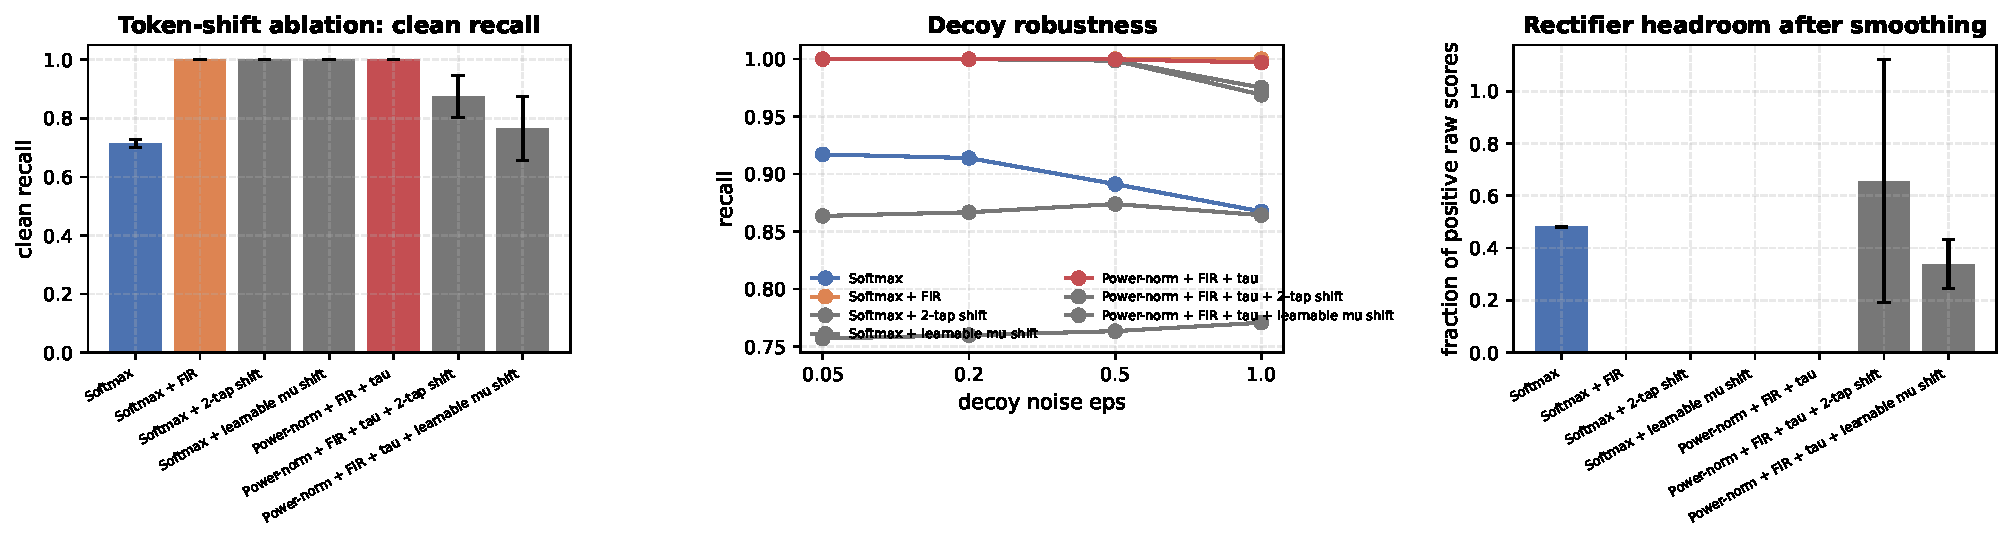
\includegraphics[width=0.98\textwidth]{figures/fig13_token_shift_ablation.pdf}
\caption{Token-shift ablation on the legacy protocol. Left: clean recall per variant. Middle: recall against the decoy-noise level. Right: the fraction of positive raw scores, i.e.\ the headroom the rectifier has left after smoothing. Bars and curves are means over $n=3$ seeds; error bars are the standard deviation over the same seeds. Source: \texttt{results/exp6\_token\_shift\_ablation.json} (\texttt{partA\_legacy.summary}).}
\label{fig:13-token-shift-ablation}
\end{figure}



\subsection{Experiment 4f-A/4g: Width Envelope and the Tau Fixed Point}

The pathology amplifies with width rather than attenuating (ladder $d \in \{16, 24, 32, 48, 64, 96, 128\}$, identical recipe, 3 seeds; \texttt{exp4f\_scaleout.py} Part A and \texttt{exp4g\_tau\_scaling\_law.py}; Fig.~\ref{fig:5-width-envelope} and Fig.~\ref{fig:6-tau-scaling-ladder}; Table~\ref{tab:width-envelope} lists the ladder values). \texttt{sm\_fir} holds $100.0\%$ at every width (its raw shift drifts mildly, $-14 \to -27$); uncalibrated \texttt{pn\_fir} raw magnitudes diverge to tens and hundreds with seed-divergent signs ($\mu_S = -20\dots-144$, $\sigma_S$ up to $\sim$300), and \texttt{pn\_fir\_tau} converges fully only at $d \in \{32, 48, 64\}$ (collapsing to $52.6\%$ at $d{=}128$; partial at 16/24, stochastic at 96/128). A linear drift-cancellation law $\tau^*(d) = a\cdot(-\mu_S) + b$ is rejected ($R^2 = 0.45$, slope $\approx 0$); instead the calibrated fixed point is width-invariant ($\tau^* \in [-1.4, -0.7]$ wherever convergence happens) while only its basin from $\tau_0 = 0$ collapses. Initializing the predicted $\tau_0 = -1.02$ rescues $d{=}128$ on all 3 seeds ($100.0\%$, equilibria $-1.19$/$-1.16$/$-1.16$) --- a dead-row basin problem at initialization, not a representational wall. Practical rule: start $\tau$ negative at width. (The H-gap diagnostic, $H_{\text{noise}} - H_{\text{match}}$, is $\approx 0$ at every width including converged ones --- uninformative under $p{=}10$ sharpening, a negative result on our own design.)

\begin{figure}[ht!]
\centering
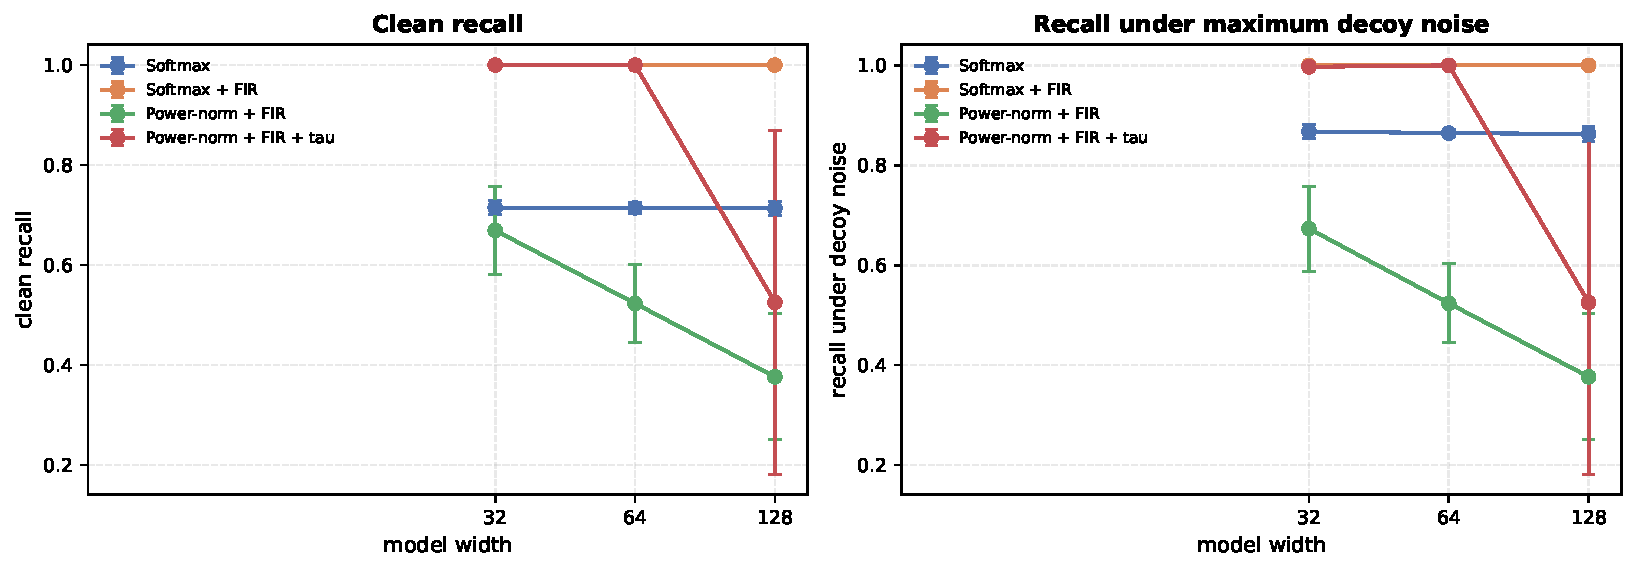
\includegraphics[width=0.98\textwidth]{figures/fig5_width_envelope.pdf}
\caption{Width envelope of the four attention variants on the legacy task. Left: clean recall; right: recall under the strongest decoy noise. Points are means over $n=3$ seeds; error bars are the standard deviation over the same seeds. Source: \texttt{results/exp4f\_scaleout.json} (\texttt{partA.arms.<arm>.by\_width.<width>}).}
\label{fig:5-width-envelope}
\end{figure}

\begin{figure}[ht!]
\centering
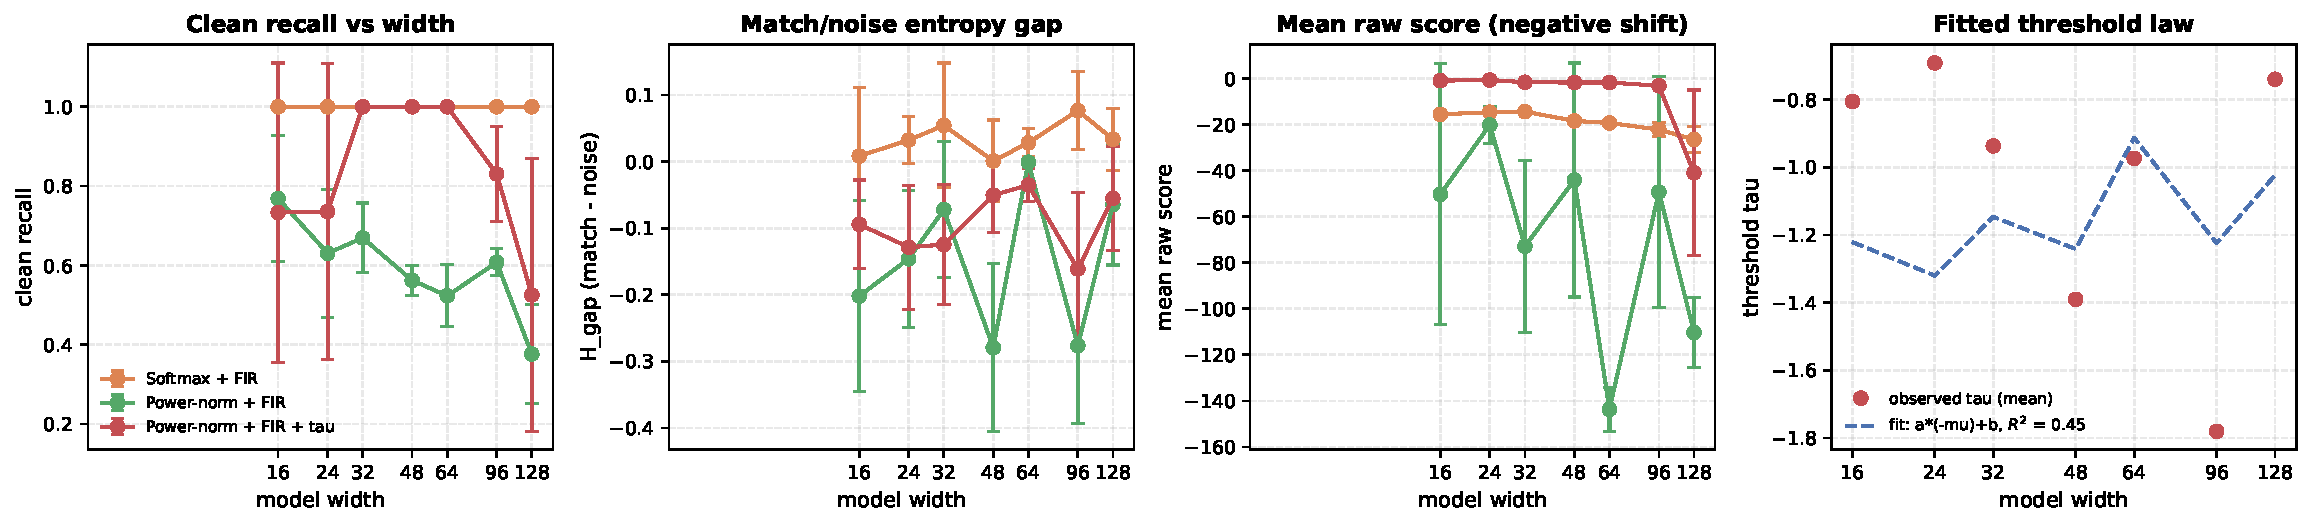
\includegraphics[width=0.98\textwidth]{figures/fig6_tau_scaling_ladder.pdf}
\caption{Behaviour of the three filtered variants across a seven-point width ladder, with the fitted threshold law. From left to right: clean recall, the match/noise entropy gap, the mean raw score, and the learned threshold against the fitted law $\tau = a\cdot(-\mu_S) + b$ ($R^2 = 0.45$, fitted on widths 32, 48, 64). Points are means over $n=3$ seeds; error bars are the standard deviation over the same seeds. Source: \texttt{results/exp4g\_tau\_scaling\_law.json} (\texttt{ladder}, \texttt{fit}).}
\label{fig:6-tau-scaling-ladder}
\end{figure}

\begin{table}[ht!]
\centering
\caption{Experiment 4f-A: width envelope of the four attention variants on the legacy task (ladder $d \in \{16, 24, 32, 48, 64, 96, 128\}$, $n=3$ seeds). $\mu_S$ is the mean raw score of the uncalibrated \texttt{pn\_fir} arm, $\tau^*$ the learned threshold of \texttt{pn\_fir\_tau}, and the H-gap the match/noise entropy difference. The last two rows report the predicted negative initialisation $\tau_0 = -1.02$ and a $10\times$ smaller learning rate at $d = 128$. Source: \texttt{results/exp4f\_scaleout.json} and \texttt{results/exp4g\_tau\_scaling\_law.json}.}
\label{tab:width-envelope}
\scriptsize
\setlength{\tabcolsep}{2.2pt}
\begin{tabular}{lcccccc}
\toprule
Width $d$ & \texttt{sm\_fir} clean & \texttt{pn\_fir} clean & \texttt{pn\_fir} raw $\mu_S$ & \texttt{pn\_fir\_tau} clean & \texttt{pn\_fir\_tau} $\tau^*$ & H-gap (tau arm) \\
\midrule
16 & $100.0$ & $76.9$ & $-50.3$ & $73.3$ & $-0.81 \pm 0.60$ & $-0.09$ \\
24 & $100.0$ & $63.1$ & $-20.2$ & $73.6$ & $-0.69 \pm 0.52$ & $-0.13$ \\
32 & $100.0$ & $66.9$ & $-72.9$ & $100.0$ & $-0.94 \pm 0.02$ & $-0.13$ \\
48 & $100.0$ & $56.2$ & $-44.1$ & $100.0$ & $-1.39 \pm 0.48$ & $-0.05$ \\
64 & $100.0$ & $52.3$ & $-143.7$ & $100.0$ & $-0.97 \pm 0.05$ & $-0.04$ \\
96 & $100.0$ & $60.8$ & $-49.3$ & $83.1$ & $-1.78 \pm 0.74$ & $-0.16$ \\
128 & $100.0$ & $37.7$ & $-110.4$ & $52.6$ & $-0.74 \pm 0.19$ & $-0.06$ \\
128, $\tau_0 = -1.02$ (predicted) & --- & --- & --- & \textbf{$100.0$} & $-1.17 \pm 0.02$ & $-0.02$ \\
128, lr $= 10^{-3}$ & $100.0$ & --- & --- & $91.0 \pm 12.8$ & $-0.60 \pm 0.14$ & --- \\
\bottomrule
\end{tabular}
\end{table}



\subsection{Experiment 3: 31-Configuration Sweep of $(\tau_0, \gamma, \text{silence\_mode})$}

Table~\ref{tab:exp3} and Figure~\ref{fig:silence}b summarize the 31-configuration sweep across threshold initialization $\tau_0$, gate constant $\gamma$, and gating mode (\texttt{peak} vs.\ \texttt{mass\_relu}). Initializing $\tau_0 = +0.5$ causes immediate ReLU starvation ($\text{clean} = 20.6\%$), while $\tau_0 = 0.0$ with \texttt{peak} gating ($\gamma \in [0.1, 0.5]$) achieves $100.0\%$ recall and strong silence ($\text{gap} = +0.572$ at $\gamma=0.10$ and $+0.432$ at $\gamma=0.50$ on seed 1234). In contrast, \texttt{mass\_relu} ($\text{gap} \le +0.010$) and \texttt{pn\_fir\_c} on positive-only training ($\text{gap} \le +0.021$, because uncalibrated noise rows have large within-row dispersion $\max_j S_{t,j} - \mu_t \gg \gamma$) fail to suppress noise across all $\gamma$.

\begin{table}[ht!]
\centering
\caption{Experiment 3: Representative configurations from the 31-point $(\tau_0, \gamma, \text{mode})$ sweep. Source: \texttt{results/exp3\_sweep\_tau\_gate.json}.}
\label{tab:exp3}
\scriptsize
\setlength{\tabcolsep}{2.2pt}
\begin{tabular}{llccccccccc}
\toprule
Stack and Mode & $\tau_0$ & $\gamma$ & Clean & $\sum W_m$ & $\sum W_n$ & Gap & $\tau$ & 3-Seed Clean & 3-Seed $\sum W_n$ & 3-Seed Gap \\
\midrule
\texttt{pn\_fir\_tau} (\texttt{peak}) & $0.0$ & None & $100.0\%$ & $1.000$ & $0.752$ & $+0.228$ & $-0.320$ & $100.0\%$ & $0.717$ & $+0.282 \pm 0.045$ \\
\texttt{pn\_fir\_tau} (\texttt{peak}) & $0.0$ & $0.05$ & $100.0\%$ & $0.882$ & $0.608$ & $+0.221$ & $-0.453$ & $100.0\%$ & $0.628$ & $+0.197 \pm 0.054$ \\
\textbf{\texttt{pn\_fir\_tau} (\texttt{peak})} & $\mathbf{0.0}$ & $\mathbf{0.10}$ & $\mathbf{100.0\%}$ & $\mathbf{0.572}$ & $\mathbf{0.000}$ & $\mathbf{+0.572}$ & $\mathbf{-0.501}$ & $\mathbf{100.0\%}$ & $\mathbf{0.336}$ & $\mathbf{+0.373 \pm 0.180}$ \\
\texttt{pn\_fir\_tau} (\texttt{peak}) & $0.0$ & $0.20$ & $100.0\%$ & $0.752$ & $0.501$ & $+0.211$ & $-0.696$ & $100.0\%$ & $0.583$ & $+0.129 \pm 0.070$ \\
\textbf{\texttt{pn\_fir\_tau} (\texttt{peak})} & $\mathbf{0.0}$ & $\mathbf{0.50}$ & $\mathbf{100.0\%}$ & $\mathbf{0.436}$ & $\mathbf{0.003}$ & $\mathbf{+0.432}$ & $\mathbf{-0.940}$ & $\mathbf{100.0\%}$ & $\mathbf{0.375}$ & $\mathbf{+0.191 \pm 0.171}$ \\
\texttt{pn\_fir\_tau} (\texttt{peak}) & $-0.5$ & $0.50$ & $100.0\%$ & $0.672$ & $0.433$ & $+0.193$ & $-1.159$ & $100.0\%$ & $0.484$ & $+0.165 \pm 0.029$ \\
\texttt{pn\_fir\_tau} (\texttt{peak}) & $-1.0$ & $0.50$ & $100.0\%$ & $0.724$ & $0.611$ & $+0.108$ & $-1.531$ & $100.0\%$ & $0.593$ & $+0.122 \pm 0.019$ \\
\texttt{pn\_fir\_tau} (\texttt{peak}) & $+0.5$ & $0.50$ & $20.9\%$ & $0.000$ & $0.000$ & $+0.000$ & $+0.500$ & $20.6\%$ & $0.000$ & $+0.000 \pm 0.000$ \\
\texttt{pn\_fir\_c} (\texttt{peak}) & $0.0$ & $0.50$ & $100.0\%$ & $0.947$ & $0.946$ & $+0.021$ & N/A & $100.0\%$ & $0.938$ & $+0.017 \pm 0.004$ \\
\texttt{pn\_fir\_tau} (\texttt{mass\_relu}) & $0.0$ & $0.50$ & $100.0\%$ & $0.847$ & $0.851$ & $-0.001$ & $-0.481$ & $100.0\%$ & $0.815$ & $+0.010 \pm 0.008$ \\
\texttt{pn\_fir\_tau} (\texttt{mass\_relu}) & $0.0$ & $1.00$ & $100.0\%$ & $0.793$ & $0.784$ & $+0.003$ & $-0.613$ & $100.0\%$ & $0.776$ & $+0.008 \pm 0.006$ \\
\bottomrule
\end{tabular}
\end{table}

\begin{figure}[ht!]
\centering
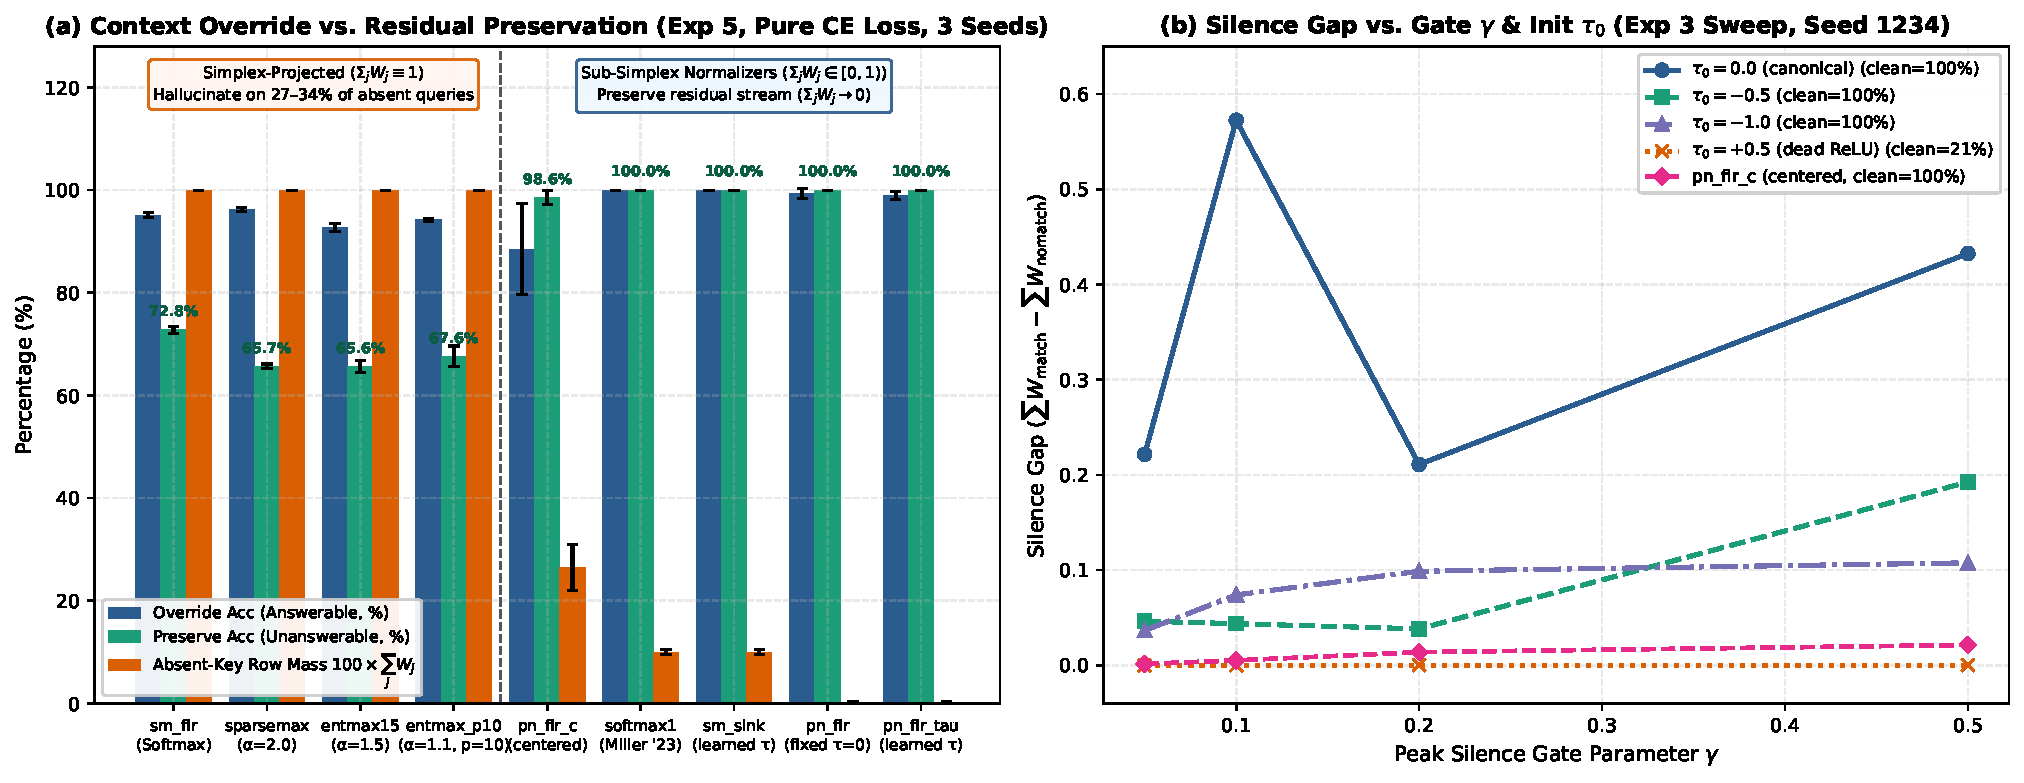
\includegraphics[width=0.98\textwidth]{figures/fig3_selective_silence.pdf}
\caption{Context override vs.\ residual stream preservation across simplex and sub-simplex normalizers under pure Cross-Entropy loss (Exp~5, left), and silence gap vs.\ gate $\gamma$ and initialization $\tau_0$ (Exp~3 sweep, right). Source: \texttt{results/exp5\_abstention\_and\_entmax.json} and \texttt{results/exp3\_sweep\_tau\_gate.json}.}
\label{fig:silence}
\end{figure}

\subsection{Experiment 5: Context Override vs.\ Residual Stream Preservation Against \texttt{Sparsemax}, \texttt{Entmax}, and \texttt{Softmax Sinks} Under Pure Cross-Entropy Loss}

{\sloppy
To test whether sub-simplex selective silence yields a concrete end-to-end task advantage over simplex normalizers (\texttt{sm\_fir}, \texttt{Sparsemax} \cite{martins2016sparsemax}, and $\alpha$-\texttt{Entmax} \cite{peters2019sparse}~\cite{correia2019adaptively}), row-mean-centered power-norm (\texttt{pn\_fir\_c}), and virtual-sink Softmax (\texttt{softmax1\_fir}, \texttt{softmax\_sink\_fir}) \textbf{under 100\% pure task Cross-Entropy loss with zero auxiliary attention regularization}, Experiment~5 (\texttt{exp5\_abstention\_and\_entmax.py}) evaluates a topic-coherent document residual stream task ($T=48$, $M=3$ pairs $(k_m, v_m) \in \{0..7\}^2$, filler tokens carrying topic values from $v_{\text{sub}}$, and query residual update $y = V(v_{\text{default}}) + 2.5 \sum_{j < 47} W_{\text{query}, j} V_j$ where $v_{\text{default}} \notin v_{\text{sub}}$). On 50\% of queries ($k^*$ present), the head must override $v_{\text{default}}$ with $v^*$; on 50\% of queries ($k^*$ absent), the head must stay silent ($\sum_j W_{\text{query}, j} \to 0$) to preserve $v_{\text{default}}$.\par}

\begin{table}[ht!]
\centering
\caption{Experiment 5: Context Override vs.\ Residual Preservation under pure Cross-Entropy loss (3 seeds: \texttt{1234, 2025, 3141}, mean $\pm$ std). All 9 models use the 7-tap causal FIR filter on $K$. Source: \texttt{results/exp5\_abstention\_and\_entmax.json}.}
\label{tab:exp5}
\scriptsize
\setlength{\tabcolsep}{2.2pt}
\begin{tabular}{llcccccccc}
\toprule
Family & Model & Overall (\%) & Overr. (\%) & Pres. (\%) & Hall. (\%) & $\sum W_a$ & $\sum W_u$ & Gap & $W_{t, j^*+1}$ \\
\midrule
Simplex & \texttt{sm\_fir} & $84.0 \pm 0.6$ & $95.1 \pm 0.5$ & $72.8 \pm 0.7$ & $\mathbf{27.2 \pm 0.7}$ & $1.000$ & $1.000$ & $+0.000$ & $0.538$ \\
Simplex & \texttt{sparsemax\_fir} ($\alpha=2.0$) & $80.9 \pm 0.2$ & $96.2 \pm 0.4$ & $65.7 \pm 0.4$ & $\mathbf{34.3 \pm 0.4}$ & $1.000$ & $1.000$ & $+0.000$ & $0.604$ \\
Simplex & \texttt{entmax15\_fir} ($\alpha=1.5$) & $79.2 \pm 0.8$ & $92.7 \pm 0.8$ & $65.6 \pm 1.1$ & $\mathbf{34.4 \pm 1.1}$ & $1.000$ & $1.000$ & $+0.000$ & $0.593$ \\
Simplex & \texttt{entmax\_p10\_fir} ($\alpha=1.1$) & $80.9 \pm 0.9$ & $94.2 \pm 0.2$ & $67.6 \pm 2.0$ & $\mathbf{32.4 \pm 2.0}$ & $1.000$ & $1.000$ & $+0.000$ & $0.560$ \\
\midrule
Centered & \texttt{pn\_fir\_c} & $93.5 \pm 5.1$ & $88.5 \pm 8.9$ & $98.6 \pm 1.3$ & $1.4 \pm 1.3$ & $0.716$ & $0.265$ & $+0.451$ & $0.577$ \\
Virtual Sink & \texttt{softmax1\_fir} ($\tau=0$) & $\mathbf{100.0 \pm 0.0}$ & $\mathbf{100.0 \pm 0.0}$ & $\mathbf{100.0 \pm 0.0}$ & $\mathbf{0.0 \pm 0.0}$ & $0.863$ & $0.100$ & $+0.764$ & $0.776$ \\
Virtual Sink & \texttt{softmax\_sink\_fir} ($\tau$) & $\mathbf{100.0 \pm 0.0}$ & $\mathbf{100.0 \pm 0.0}$ & $\mathbf{100.0 \pm 0.0}$ & $\mathbf{0.0 \pm 0.0}$ & $0.864$ & $0.100$ & $+0.764$ & $0.775$ \\
Sub-Simplex & \texttt{pn\_fir} ($\tau=0, p=10$) & $99.7 \pm 0.5$ & $99.4 \pm 0.9$ & $\mathbf{100.0 \pm 0.0}$ & $\mathbf{0.0 \pm 0.0}$ & $0.747$ & $\mathbf{0.002}$ & $+0.745$ & $0.724$ \\
Sub-Simplex & \textbf{\texttt{pn\_fir\_tau} ($\tau, p=10$)} & $\mathbf{99.5 \pm 0.4}$ & $\mathbf{99.0 \pm 0.7}$ & $\mathbf{100.0 \pm 0.0}$ & $\mathbf{0.0 \pm 0.0}$ & $0.744$ & $\mathbf{0.002}$ & $\mathbf{+0.742}$ & $0.716$ \\
\bottomrule
\end{tabular}
\end{table}

Table~\ref{tab:exp5} and Figure~\ref{fig:silence}a establish four key findings: (1) all four simplex normalizers fail residual preservation ($27.2\%\text{--}34.4\%$ hallucination rate), with \texttt{sparsemax\_fir} and \texttt{entmax} performing even worse than \texttt{sm\_fir} because sparse simplex projection concentrates weight onto a single mismatching topic token; (2) under pure Cross-Entropy loss with 50\% unanswerable queries, \texttt{pn\_fir\_tau} places unanswerable raw score peaks below $\tau = +0.011 \pm 0.020$ ($\max_j S^{\text{raw}}_{\text{unans}} = -0.175 \pm 0.070 < \tau$, while $\max_j S^{\text{raw}}_{\text{ans}} = +1.548 \pm 0.281 \gg \tau$), achieving $100.0\% \pm 0.0\%$ residual preservation ($0.0\%$ hallucination rate) and $\sum W_{\text{unans}} = 0.002 \pm 0.002$ (note that because 50\% of training examples are unanswerable, $W_Q, W_K$ naturally center unanswerable scores below zero, so fixed $\tau=0$ \texttt{pn\_fir} performs equally well here at $99.7\% \pm 0.5\%$, whereas learnable $\tau$ is essential when training is dominated by positive retrieval as in Exp~1--2 or multi-layer LM in Exp~4); (3) \texttt{pn\_fir\_c} shrinks $\|Q_{\text{query}}\|_2$ on unanswerable rows to reach $\sum W_{\text{unans}} = 0.265 \pm 0.045$ ($\text{gap} = +0.451 \pm 0.032$), but still leaks $\approx 124\times$ more residual noise than \texttt{pn\_fir\_tau} while degrading answerable override accuracy ($88.5\% \pm 8.9\%$ vs.\ $99.0\% \pm 0.7\%$); and (4) comparing \texttt{pn\_fir\_tau} against virtual-sink Softmax (\texttt{softmax1\_fir}, \texttt{softmax\_sink\_fir}) reveals a clean trade-off: virtual-sink Softmax achieves slightly higher discrete answerable override accuracy ($100.0\% \pm 0.0\%$ vs.\ $99.0\% \pm 0.7\%$) and higher active mass ($\sum W_{\text{ans}} = 0.863\text{--}0.864$ vs.\ $0.744$), whereas \texttt{pn\_fir\_tau} achieves $50\times$ lower continuous residual-stream contamination on unanswerable queries ($\sum W_{\text{unans}} = 0.002 \pm 0.002$ vs.\ $0.100 \pm 0.005$).

\subsection{Experiment 4: 6-Layer Causal Language Modeling on WikiText-2 and Fused Triton Benchmarks}

We evaluate a 6-layer Pre-LN Transformer on word-level WikiText-2 ($V=23,168, D=64, H=4, d_{\text{ff}}=256, N=256, B=64$, tied embeddings: $1,482,752 \text{ (tok\_emb)} + 16,384 \text{ (pos\_emb)} + 6 \times 49,728 \text{ (298,368)} + 128 \text{ (ln\_f)} = 1,797,632$ base parameters; $+6$ scalar $\tau_\ell$ parameters in \texttt{pn\_fir\_tau} for $1,797,638$ total). In IEEE-754 \texttt{FP32} parity checks (\texttt{allow\_tf32=False}, reference norms $\|y\|_\infty = 0.5441, \|dx\|_\infty = 2.1698, |d\tau| = 7.0289$), both \texttt{PnFirTauTritonMHA} ($\text{out\_max\_diff} = 2.38\times 10^{-7}$ [rel $4.38\times 10^{-7}$], $\text{dx\_max\_diff} = 1.16\times 10^{-6}$ [rel $5.36\times 10^{-7}$], $\text{dtau\_diff} = 3.91\times 10^{-5}$ [rel $5.56\times 10^{-6}$]) and \texttt{PnFirTauFlashMHA} ($\text{out\_max\_diff} = 2.38\times 10^{-7}$, $\text{dx\_max\_diff} = 1.32\times 10^{-6}$ [rel $6.08\times 10^{-7}$], $\text{dtau\_diff} = 4.01\times 10^{-5}$ [rel $5.70\times 10^{-6}$]) closely match eager PyTorch. Table~\ref{tab:exp4}, Table~\ref{tab:exp4_mha}, Table~\ref{tab:exp4_skip}, and Figure~\ref{fig:wikitext} present the full benchmark suite.

\begin{table}[ht!]
\centering
\caption{Experiment 4: WikiText-2 6-layer Language Model benchmarks ($B=64, N=256$, RTX 3060). Suites 1--3 and suite 2s are defined in the text; suite 3 is precision-controlled across 3 seeds; suite 2s (D=256) is a single-seed pilot; step times are omitted for suite 3 and suite 2s (see notes below). Source: \texttt{results/exp4\_wikitext2\_lm.json}.}
\label{tab:exp4}
\scriptsize
\setlength{\tabcolsep}{3.0pt}
\begin{tabular}{llcccc}
\toprule
Suite & Variant & Precision & ms/step & Rel.\ Time & VRAM (GB) \\
\midrule
suite 1: Speed/VRAM & \texttt{softmax} & \texttt{BF16+TF32} & $97.70$ & $1.000\times$ & $5.16$ \\
suite 1: Speed/VRAM & \texttt{sm\_fir} (FIR) & \texttt{BF16+TF32} & $99.21$ & $1.016\times$ & $5.17$ \\
suite 1: Speed/VRAM & \texttt{pn\_fir\_tau} (Eager) & \texttt{BF16+TF32} & $164.44$ & $1.683\times$ & $6.11$ \\
suite 1: Speed/VRAM & \textbf{\texttt{pn\_fir\_tau\_triton}} & \texttt{BF16+TF32} & $\mathbf{75.74}$ & $\mathbf{0.775\times}$ & $\mathbf{4.97}$ \\
suite 1: Speed/VRAM & \textbf{\texttt{pn\_fir\_tau\_flash}} & \texttt{BF16+TF32} & $\mathbf{66.80}$ & $\mathbf{0.684\times}$ & $\mathbf{4.52}$ \\
suite 1: Speed/VRAM & \texttt{softmax} & \texttt{FP32+TF32} & $140.92$ & $1.000\times$ & $6.92$ \\
suite 1: Speed/VRAM & \texttt{sm\_fir} (FIR) & \texttt{FP32+TF32} & $143.76$ & $1.020\times$ & $6.94$ \\
suite 1: Speed/VRAM & \texttt{pn\_fir\_tau} (Eager) & \texttt{FP32+TF32} & $244.17$ & $1.733\times$ & $8.82$ \\
suite 1: Speed/VRAM & \textbf{\texttt{pn\_fir\_tau\_triton}} & \texttt{FP32+TF32} & $\mathbf{120.43}$ & $\mathbf{0.855\times}$ & $\mathbf{6.92}$ \\
suite 1: Speed/VRAM & \textbf{\texttt{pn\_fir\_tau\_flash}} & \texttt{FP32+TF32} & $\mathbf{105.84}$ & $\mathbf{0.751\times}$ & $\mathbf{6.10}$ \\
\bottomrule
\end{tabular}
\vspace{0.6em}
\setlength{\tabcolsep}{2.2pt}
\begin{tabular}{llcccccc}
\toprule
Suite & Variant & Precision & Params & Train & Val & Test & Leak \\
\midrule
suite 2 & \texttt{softmax} & \texttt{BF16+TF32} & $1,797,632$ & $654.23$ & $547.33$ & $515.55$ & $5.16$ \\
suite 2 & \texttt{sm\_fir} & \texttt{BF16+TF32} & $1,797,632$ & $652.97$ & $547.29$ & $515.18$ & $5.17$ \\
suite 2 & \texttt{pn\_fir\_tau} (Eager) & \texttt{BF16+TF32} & $1,797,638$ & $653.17$ & $546.75$ & $515.56$ & $6.11$ \\
suite 2 & \textbf{\texttt{pn\_fir\_tau\_triton}} & \texttt{BF16+TF32} & $1,797,638$ & $652.00$ & $545.78$ & $515.40$ & $\mathbf{4.97}$ \\
suite 2 & \textbf{\texttt{pn\_fir\_tau\_flash}} & \texttt{BF16+TF32} & $1,797,638$ & $653.54$ & $546.78$ & $516.11$ & $\mathbf{4.52}$ \\
suite 2s & \texttt{softmax} & \texttt{BF16+TF32} & $10,795,008$ & $441.16$ & $411.03$ & $379.83$ & ---$^\ddagger$ \\
suite 2s & \texttt{sm\_fir} & \texttt{BF16+TF32} & $10,795,008$ & $416.71$ & $390.09$ & $359.48$ & ---$^\ddagger$ \\
suite 2s & \texttt{pn\_fir\_tau} (+6 $\tau$) & \texttt{BF16+TF32} & $10,795,014$ & $428.52$ & $409.33$ & $377.36$ & ---$^\ddagger$ \\
suite 3 & \texttt{softmax} & \texttt{BF16+TF32} & $1,797,632$ & $77.93 \pm 0.41$ & $124.37 \pm 0.26$ & $117.13 \pm 0.04$ & --- \\
suite 3 & \textbf{\texttt{pn\_fir\_tau}} & \texttt{BF16+TF32} & $\mathbf{1,797,638}$ & $78.30 \pm 0.45$ & $\mathbf{122.15 \pm 0.72}$ & $\mathbf{114.80 \pm 0.49}$ & --- \\
\bottomrule
\end{tabular}
\paragraph*{Precision-controlled 50k, 3 seeds.} Both suite 3 runs use \texttt{BF16+TF32} across 3 seeds per variant (softmax: one seed-42 run plus seeds 43--44; pn: one seed-42 run plus seeds 43--44; \texttt{results/exp4d\_softmax\_50k\_bf16.json}, \texttt{results/exp4e\_multiseed\_50k.json}), giving a matched 50k gap of $-2.22 \pm 0.46$ val / $-2.33 \pm 0.49$ test PPL for \texttt{pn\_fir\_tau}, holding on all 3 seeds (per-seed val gaps $-2.26$/$-2.76$/$-1.64$).

\paragraph*{suite 2s notes.} $^\dagger$Effective wall-clock per step including eval amortization ($725/1121/789$~ms for softmax/sm\_fir/pn\_fir\_tau). A pure-step bench was attempted and abandoned: under WSL GPU-PV paging the FP32 suite crawls and eager \texttt{pn\_fir\_tau} OOMs the bench harness on backward. $^\ddagger$Peak VRAM under WSL paging is non-comparable (measured $14.1/14.2/18.2$~GB on a 12~GB card) and omitted; a native-Linux measurement is left for future work.


\end{table}

\begin{table}[ht!]
\centering
\caption{Quantization Hygiene: INT8 Activation Noise, Attention-Sink Mass, and Residual Outliers (Exp~4h). Per-token symmetric INT8 quantize-dequantize on every \texttt{nn.Linear} input (activation-only emulation, weights kept in fp), evaluated on the trained checkpoints. Sink mass is the mean attention mass on position 0 over the six layers. Source: \texttt{results/exp4h\_int8\_quant.json}.}
\label{tab:int8-hygiene}
\scriptsize
\setlength{\tabcolsep}{2.2pt}
\begin{tabular}{lcccccc}
\toprule
Model & FP test PPL & INT8-sim PPL & Degrad. & Sink mass pos-0 & Resid. absmax & Resid. kurtosis \\
\midrule
D=64 \texttt{softmax} 50k & $117.15$ & $117.27$ & $+0.10\%$ & $0.0177$ & $5.03$ & $4.17$ \\
D=64 \texttt{pn\_fir\_tau} 50k & $114.25$ & $114.35$ & $+0.09\%$ & $0.0031$ & $4.08$ & $4.22$ \\
D=256 \texttt{softmax} 2.4k & $379.81$ & $380.96$ & $+0.30\%$ & $0.0122$ & $207.3$ & $85.6$ \\
D=256 \texttt{sm\_fir} 2.4k & $359.47$ & $360.75$ & $+0.36\%$ & $0.0191$ & $219.7$ & $119.7$ \\
D=256 \texttt{pn\_fir\_tau} 2.4k & $377.37$ & $378.88$ & $+0.40\%$ & $0.0013$ & $176.5$ & $78.5$ \\
\bottomrule
\end{tabular}
\end{table}

\paragraph*{Quantization hygiene (Exp~4h).} Per-token symmetric INT8 quantize-dequantize on every \texttt{nn.Linear} input (Table~\ref{tab:int8-hygiene}) costs $<0.5\%$ test PPL for every variant (D=64: $117.27$ vs.\ $117.15$ softmax, $114.35$ vs.\ $114.25$ pn; D=256: $+0.30$/$+0.36$/$+0.40\%$) --- no Softpick-scale low-bit win replicates at 2--11M parameters, and none is claimed. No massive sinks appear anywhere (max pos-0 mass $1.9\%$). The rectified hygiene advantage is real but conditional: \texttt{pn\_fir\_tau} carries $6$--$15\times$ less pos-0 mass ($0.0031$ vs.\ $0.0177$ at D=64; $0.0013$ vs.\ $0.0122$--$0.0191$ at D=256, decaying to $0.0001$ with depth) and $15$--$44\%$ lower kurtosis across roles under D=256 scale-up stress, closing after converged training at D=64.

\begin{table}[ht!]
\centering
\caption{Isolated 6-Layer MHA Stack and 1-Layer Kernel (\texttt{kern1}) Scaling ($D=64, H=4, d_k=16$, uniform $B_M=B_N=64$, Forward + Backward in \texttt{BF16+TF32}, 200 steps after 25 warmup, RTX 3060). Source: \texttt{results/exp4b\_mha6\_instrumentation.json}.}
\label{tab:exp4_mha}
\scriptsize
\setlength{\tabcolsep}{2.0pt}
\begin{tabular}{lccccc}
\toprule
Seq, Batch & \texttt{softmax} & \texttt{sm\_fir} & \texttt{pn} Eager & \textbf{\texttt{pn\_triton}} & \textbf{\texttt{pn\_flash}} \\
\midrule
$N=256, B=64$ & $34.26 \pm 0.69$ & $35.23 \pm 0.80$ & $101.02 \pm 1.29$ & $\mathbf{21.74 \pm 4.97}$ & $\mathbf{17.66 \pm 2.28}$ [$1.19 \pm 0.28$] \\
$N=512, B=64$ & $125.41 \pm 2.34$ & $127.52 \pm 2.04$ & $390.64 \pm 6.12$ & $\mathbf{37.76 \pm 0.94}$ & $\mathbf{20.60 \pm 2.73}$ [$2.05 \pm 0.14$] \\
$N=1024, B=64$ & OOM & OOM & OOM & $\mathbf{132.23 \pm 1.01}$ & $\mathbf{46.77 \pm 0.54}$ [$6.17 \pm 0.20$] \\
$N=1024, B=16$ & $126.35 \pm 0.67$ & $127.76 \pm 0.34$ & $393.42 \pm 0.43$ & $\mathbf{34.33 \pm 0.52}$ & $\mathbf{18.13 \pm 2.44}$ [$1.98 \pm 0.17$] \\
\bottomrule
\end{tabular}
\vspace{0.5em}
{\footnotesize (a) step time (ms/step, fwd+bwd); (b) peak VRAM (MB). Per-row speedups ($4.65\times$--$21.70\times$) are reported in \S3.5.}
\vspace{0.5em}
\setlength{\tabcolsep}{2.6pt}
\begin{tabular}{lccccc}
\toprule
Seq, Batch & \texttt{softmax} & \texttt{sm\_fir} & \texttt{pn} Eager (MB) & \textbf{\texttt{pn\_triton}} (MB) & \textbf{\texttt{pn\_flash}} (MB) \\
\midrule
$N=256, B=64$ & $815.2$ & $827.5$ & $1886.9$ & $\mathbf{503.3}$ & $\mathbf{109.3}$ \\
$N=512, B=64$ & $3086.3$ & $3110.6$ & $7341.4$ & $\mathbf{1821.8}$ & $\mathbf{201.8}$ \\
$N=1024, B=64$ & OOM ($>12$~GB) & OOM ($>12$~GB) & OOM ($>12$~GB) & $\mathbf{6954.8}$ & $\mathbf{386.8}$ \\
$N=1024, B=16$ & $3028.8$ & $3040.9$ & $7268.3$ & $\mathbf{1751.3}$ & $\mathbf{109.3}$ \\
\bottomrule
\end{tabular}
\end{table}

\begin{table}[ht!]
\centering
\caption{Silent-Tile Skipping Profile ($N=1024, B=16$, $B_M=B_N=64$, Forward + Backward, 200 steps). While the isolated 1-layer kernel (\texttt{kern1}) speeds up by $1.73\times$--$1.76\times$ when whole $64\times 64$ tiles are silent ($\tau \ge +1.0$), scattered row silence ($\tau=+0.5, 69.1\%$ silent rows) leaves at least one positive entry in almost every $64\times 64$ tile. The 6-layer module is launch-serialised ($\approx$372 CUDA kernel launches per step, invariant across $\tau$ and $B \in \{4,16\}$; $\approx$52\,\textmu s per launch under WSL2 GPU-PV), so isolated-kernel savings do not translate into stack wall time; the \texttt{mha6} column here uses the original sequential protocol and its end-to-end difference is identified as a block-order artifact by the drift-controlled re-measurement (\texttt{experiments/exp4b\_mha6\_instrumentation.py}).}
\label{tab:exp4_skip}
\scriptsize
\setlength{\tabcolsep}{2.0pt}
\begin{tabular}{ccccccc}
\toprule
Threshold $\tau$ & Silent rows & Mean row mass & 1L kernel (ms) & 1L speedup & 6L module (ms) & 6L speedup \\
\midrule
$-0.5$ & $0.0\%$ & $0.655$ & $1.99 \pm 0.14$ & $1.00\times$ & $19.25 \pm 3.35$ & $1.00\times$ \\
$0.0$ & $0.3\%$ & $0.469$ & $1.94 \pm 0.15$ & $1.02\times$ & $18.77 \pm 2.90$ & $1.03\times$ \\
$+0.5$ & $69.1\%$ & $0.048$ & $1.91 \pm 0.12$ & $1.04\times$ & $18.24 \pm 2.60$ & $1.06\times$ \\
$+1.0$ & $99.9\%$ & $0.0001$ & $\mathbf{1.14 \pm 0.21}$ & $\mathbf{1.73\times}$ & $18.32 \pm 3.47$ & $1.05\times$ \\
$+1.5$ & $100.0\%$ & $0.0000$ & $\mathbf{1.13 \pm 0.20}$ & $\mathbf{1.75\times}$ & $18.07 \pm 3.11$ & $1.07\times$ \\
$+2.5$ & $100.0\%$ & $0.0000$ & $\mathbf{1.13 \pm 0.18}$ & $\mathbf{1.76\times}$ & $17.65 \pm 2.32$ & $1.09\times$ \\
\bottomrule
\end{tabular}
\end{table}

\paragraph{Drift-controlled re-measurement of the 6-layer stack.}
To separate the kernel-level saving from the stack-level wall, we re-instrumented the exact configuration of Table~\ref{tab:exp4_skip} ($N{=}1024$, $B{=}16$, \texttt{BF16} autocast, matmul \texttt{TF32} off, seed 42) with $\tau$ blocks interleaved in rotating order (three $(\tau{=}-0.5, \tau{=}{+}2.5)$ pairs, three low-start and three high-start; 25 warmup + 120 timed steps per block), CUDA-event spans around the forward residual loop and the backward pass, per-layer per-tile skip diagnostics, \texttt{torch.profiler} launch counts, and a $B \in \{16, 4\}$ workload-scaling discriminator. Table~\ref{tab:drift-ctrl} reports the outcome: the stack wall is $\tau$-flat ($-0.43 \pm 0.43$ ms, $|z| \approx 1.0$, $n = 6$ block pairs) even though the isolated kernel is not ($2.167 \pm 0.027 \to 1.464 \pm 0.032$ ms, $1.48\times$, i.e.\ $0.703 \pm 0.042$ ms per layer, $4.2$ ms over six layers), the number of CUDA kernel launches per step is invariant across $\tau$ and $B$ ($372.7$ vs.\ $372.3$), and $100.0\%$ of the $64 \times 64$ tiles are fully silent in every layer at $\tau = +2.5$ against the $46.9\%$ causal floor at $\tau = -0.5$. The launch-bound diagnosis is then confirmed by intervention: capturing the entire 6-layer forward+backward in a CUDA graph (Table~\ref{tab:cuda-graph}) amortises dispatch to a single replay and surfaces the saving in full ($12.10 \pm 0.03 \to 4.91 \pm 0.02$ ms, $\Delta = -7.20 \pm 0.02$ ms), while the eager walls measured in the same process stay $\tau$-flat ($+2.04$ ms, within drift). The design lever at this stack scale is therefore fewer launches per step (graph capture or kernel fusion), not more skipping.

\begin{table}[ht!]
\centering
\caption{Drift-Controlled Re-Measurement of the 6-Layer Stack (Exp~4b). The $\tau$ blocks are interleaved in rotating order (three $(\tau{=}-0.5, \tau{=}{+}2.5)$ pairs, three low-start and three high-start; 25 warmup + 120 timed steps per block) at $N{=}1024$, $B{=}16$, \texttt{BF16} autocast, matmul \texttt{TF32} off, seed 42, so that the wall time is measured against within-session drift instead of against the block order. Wall times, spans and kernel times are in milliseconds; the last row is the $B\,16 \to 4$ workload-scaling comparison (standard errors over the two blocks: $\tau{=}-0.5$: $19.50 \pm 0.20$ vs.\ $18.88 \pm 0.16$~ms; $\tau{=}+2.5$: $18.49 \pm 0.39$ vs.\ $19.76 \pm 0.36$~ms). Source: \texttt{results/exp4b\_mha6\_instrumentation.json}.}
\label{tab:drift-ctrl}
\scriptsize
\setlength{\tabcolsep}{1.8pt}
\begin{tabular}{lccc}
\toprule
Quantity & $\tau = -0.5$ (active) & $\tau = +2.5$ (silent) & $\Delta$ \\
\midrule
Stack wall per step (6 blocks) & $20.30 \pm 0.30$ & $19.87 \pm 0.33$ & $-0.43 \pm 0.43$ ($|z| \approx 1.0$) \\
Forward residual-loop span & $8.23$ & $8.37$ & $+0.15$ ($\tau$-invariant) \\
Backward span & $11.61$ & $10.96$ & $-0.65$ (vs.\ $4.2$ predicted) \\
Isolated kernel wall (\texttt{kern1}) & $2.167 \pm 0.027$ & $1.464 \pm 0.032$ & $-0.703 \pm 0.042$ ($1.48\times$) \\
Fully-silent $64{\times}64$ tiles/layer & $46.9\%$ & $100.0\%$ & $+53.1$ p.p. \\
CUDA kernel launches per step & $372.7$ & $372.3$ & invariant ($\approx 52\,\mu$s/launch) \\
Stack wall, $4\times$ less GPU work & $19.50$ vs.\ $18.88$ & $18.49$ vs.\ $19.76$ & $3.08\times$ / $3.23\times$ SEM \\
\bottomrule
\end{tabular}
\end{table}

\begin{table}[ht!]
\centering
\caption{Launch Amortisation Isolated by CUDA-Graph Replay (Exp~4c). The whole 6-layer forward+backward is captured in a CUDA graph, so per-step launch dispatch is replaced by a single replay; the eager walls are measured in the same process. The replay-determinism check gives a maximum relative gradient deviation of $5.5 \times 10^{-3}$ at $\tau = -0.5$ and exactly $0$ at $\tau = +2.5$. Source: \texttt{results/exp4c\_cuda\_graphs.json}.}
\label{tab:cuda-graph}
\scriptsize
\setlength{\tabcolsep}{2.4pt}
\begin{tabular}{lccc}
\toprule
Quantity (rotated interleave) & $\tau = -0.5$ (fully active) & $\tau = +2.5$ (all tiles silent) & $\Delta$ ($+2.5$ vs.\ $-0.5$) \\
\midrule
Eager stack wall (launch-bound) & $21.46 \pm 0.47$ ms & $23.50 \pm 0.68$ ms & $+2.04$ ms (within drift) \\
CUDA-graph replay wall (fwd + bwd) & $12.10 \pm 0.03$ ms & $4.91 \pm 0.01$ ms & $-7.20 \pm 0.02$ ms \\
Speed-up vs.\ eager at the same $\tau$ & $1.77\times$ & $4.79\times$ & --- \\
\bottomrule
\end{tabular}
\end{table}

\paragraph{Supporting figures for Experiment 4.} Figures~\ref{fig:7-multiseed-50k-learning-curves} and \ref{fig:8-multiseed-perplexity} show the 50k-step training curves and the per-seed perplexity of the matched precision-controlled protocol. Figure~\ref{fig:9-silence-diagnostics-by-tau} reports the per-layer silence diagnostics behind Table~\ref{tab:exp4_skip}, and Figure~\ref{fig:18-schematic-silent-tile} illustrates the silent-tile skipping mechanism. Figure~\ref{fig:10-predicted-vs-realized-saving} compares the saving predicted from the single-kernel measurement against the saving realized by the 6-layer stack, Figure~\ref{fig:11-cuda-graph-launch-amortization} isolates launch amortisation by CUDA-graph replay, and Figure~\ref{fig:14-measurement-order-drift} quantifies the measurement-order drift. Figure~\ref{fig:12-int8-outlier-sites} reports the INT8 outlier and attention-sink diagnostics of Experiment~4h.

\begin{figure}[ht!]
\centering
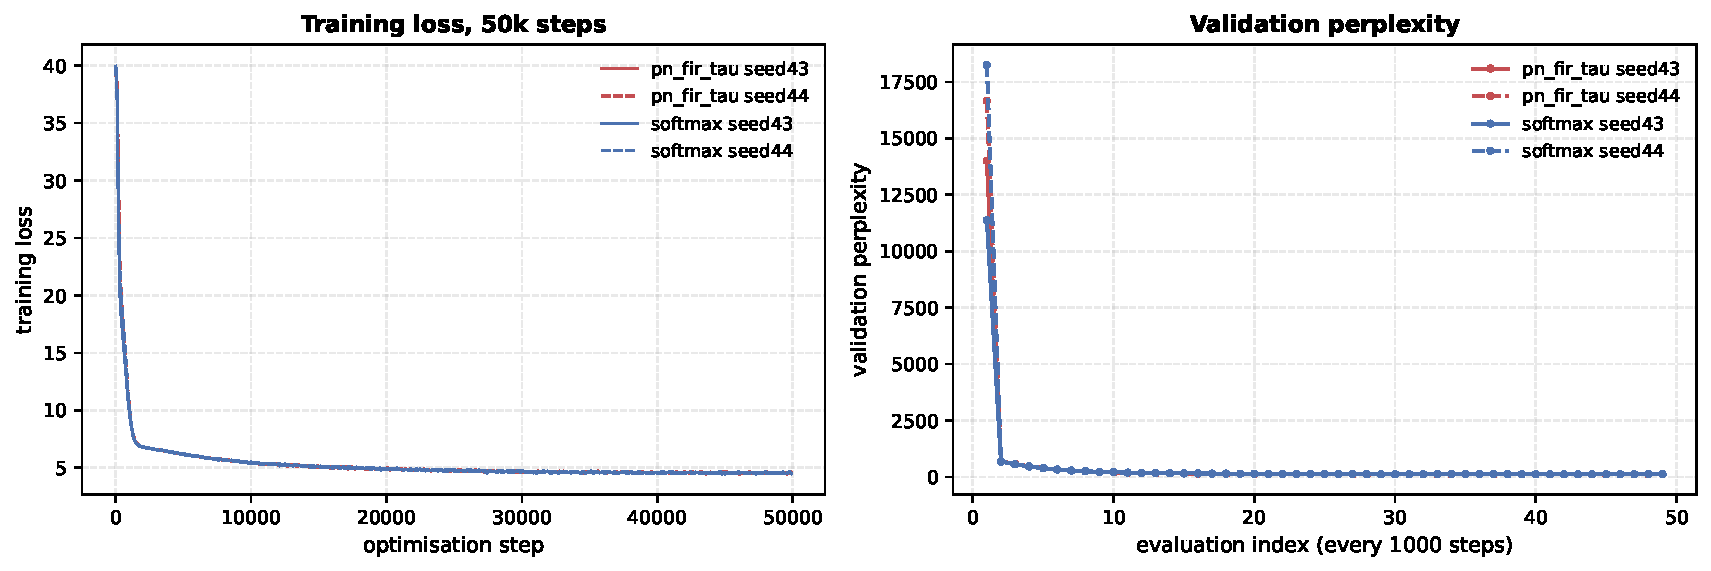
\includegraphics[width=0.98\textwidth]{figures/fig7_multiseed_50k_learning_curves.pdf}
\caption{Training history of the 50k-step runs. Left: training loss against optimisation step. Right: validation perplexity at the periodic evaluations. Curves are $n=2$ seeds per variant (seeds 43 and 44); no seed-level error band is shown, because two seeds do not support one. Source: \texttt{results/exp4e\_multiseed\_50k.json} (\texttt{runs.<variant>/<seed>.history}).}
\label{fig:7-multiseed-50k-learning-curves}
\end{figure}

\begin{figure}[ht!]
\centering
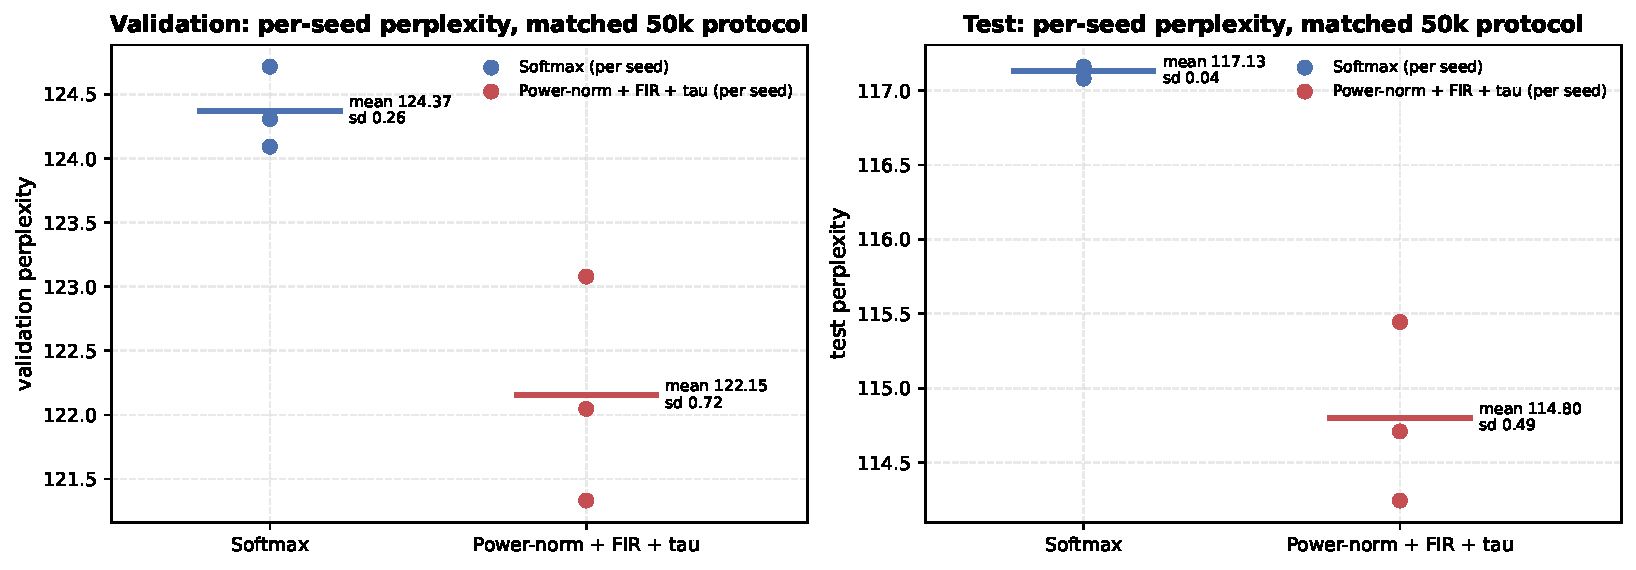
\includegraphics[width=0.98\textwidth]{figures/fig8_multiseed_perplexity.pdf}
\caption{Per-seed perplexity under the matched 50k protocol. Each dot is one seed ($n=3$ per variant); the bar is the mean over those seeds and the annotation gives the mean and the standard deviation over seeds. The seed-42 point of the rectified variant is the reference run of the matched-precision record; the two remaining seeds come from the multi-seed run. Source: \texttt{results/exp4e\_multiseed\_50k.json} and \texttt{results/exp4d\_softmax\_50k\_bf16.json}.}
\label{fig:8-multiseed-perplexity}
\end{figure}

\begin{figure}[ht!]
\centering
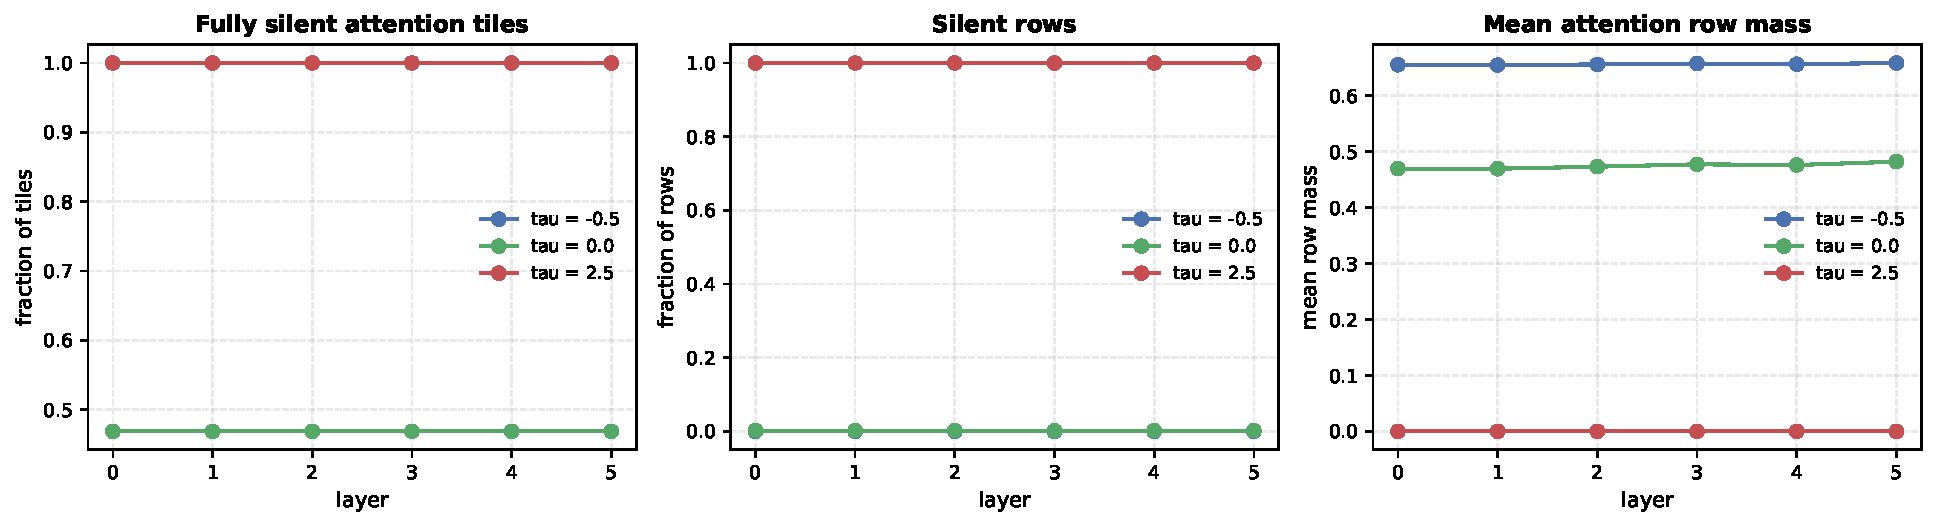
\includegraphics[width=0.98\textwidth]{figures/fig9_silence_diagnostics_by_tau.pdf}
\caption{Per-layer silence diagnostics of the 6-layer stack for three thresholds. Left: fraction of fully silent attention tiles. Middle: fraction of silent rows. Right: mean attention row mass. Single instrumented run per threshold (one run per $\tau$), so no seed spread is shown. Source: \texttt{results/exp4b\_mha6\_instrumentation.json} (\texttt{diagnostics\_per\_tau}).}
\label{fig:9-silence-diagnostics-by-tau}
\end{figure}

\begin{figure}[ht!]
\centering
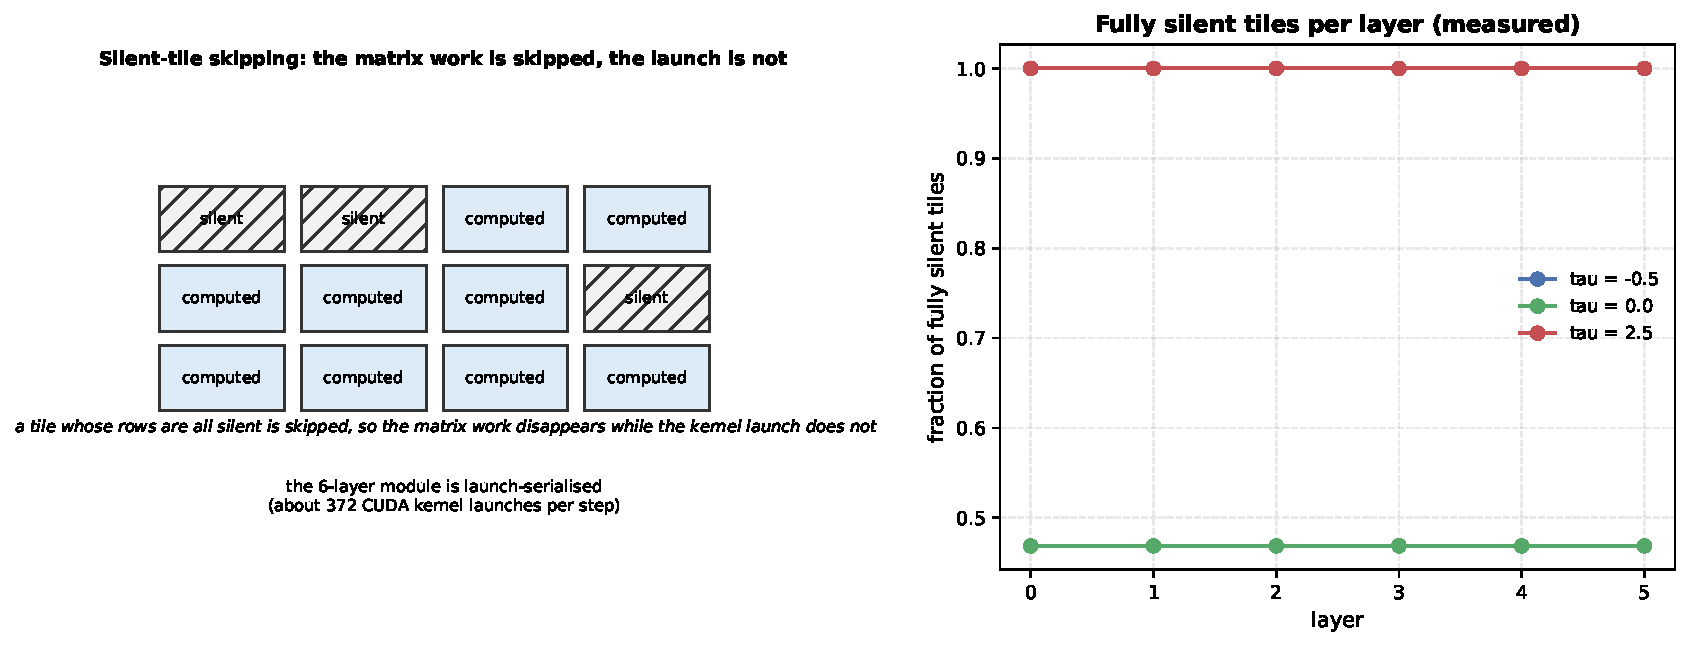
\includegraphics[width=0.98\textwidth]{figures/fig18_schematic_silent_tile.pdf}
\caption{Schematic of silent-tile skipping. Left: a tile grid in which tiles whose rows are all silent are skipped, so the matrix work disappears while the kernel launch does not; the 6-layer module is launch-serialised with about 372 CUDA kernel launches per step. Right: the measured fraction of fully silent tiles per layer and threshold. Single instrumented run per threshold. Source: \texttt{results/exp4b\_mha6\_instrumentation.json} (\texttt{diagnostics\_per\_tau}) and \texttt{src/triton\_pnfirtau.py}.}
\label{fig:18-schematic-silent-tile}
\end{figure}

\begin{figure}[ht!]
\centering
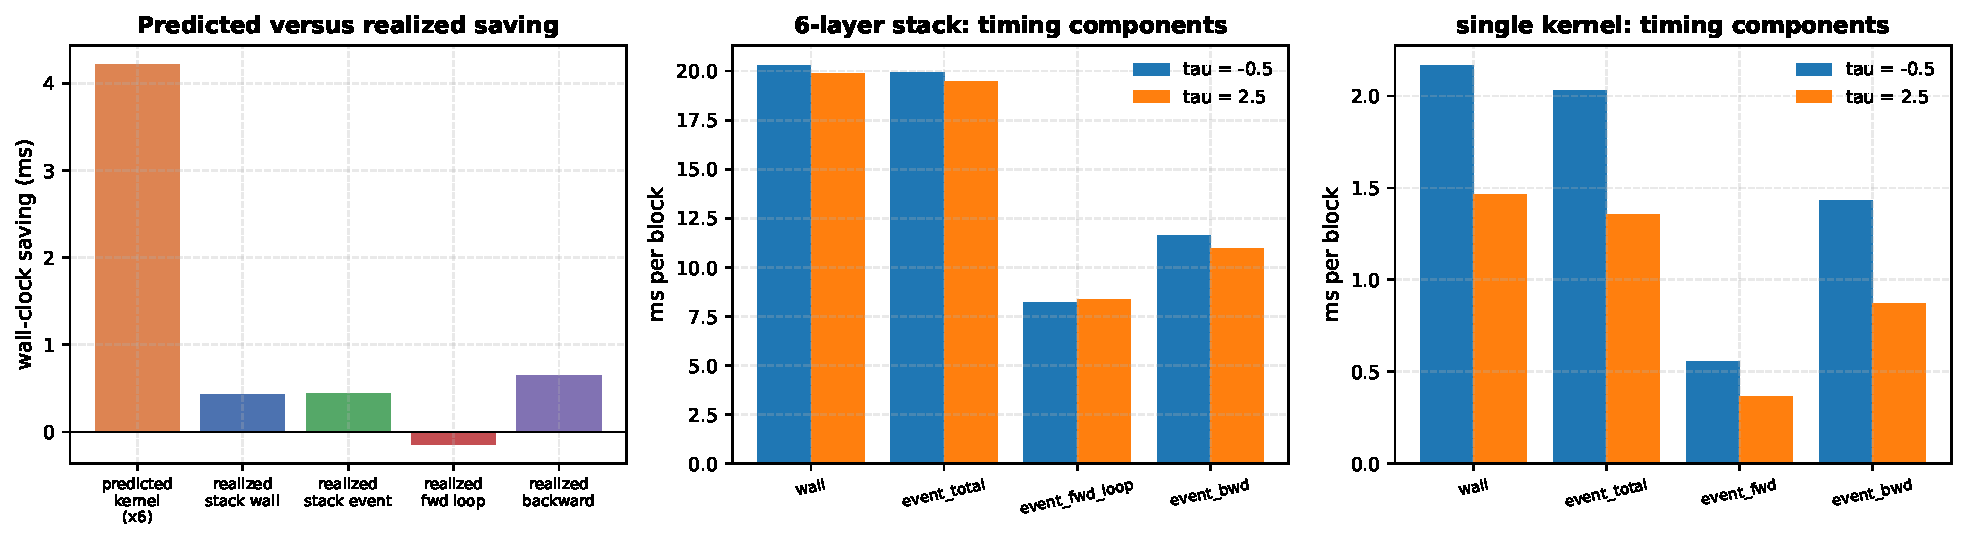
\includegraphics[width=0.98\textwidth]{figures/fig10_predicted_vs_realized_saving.pdf}
\caption{Predicted versus realized wall-clock saving. Left: the saving predicted from the single-kernel measurement against the saving actually realized by the 6-layer stack and its forward/backward split. Centre and right: timing components of the stack and of the single kernel. Single instrumented run per threshold; the error bars of the underlying block timings are reported in the text, not drawn here. Source: \texttt{results/exp4b\_mha6\_instrumentation.json} (\texttt{attribution}, \texttt{stack\_timing}, \texttt{kern1\_timing}).}
\label{fig:10-predicted-vs-realized-saving}
\end{figure}

\begin{figure}[ht!]
\centering
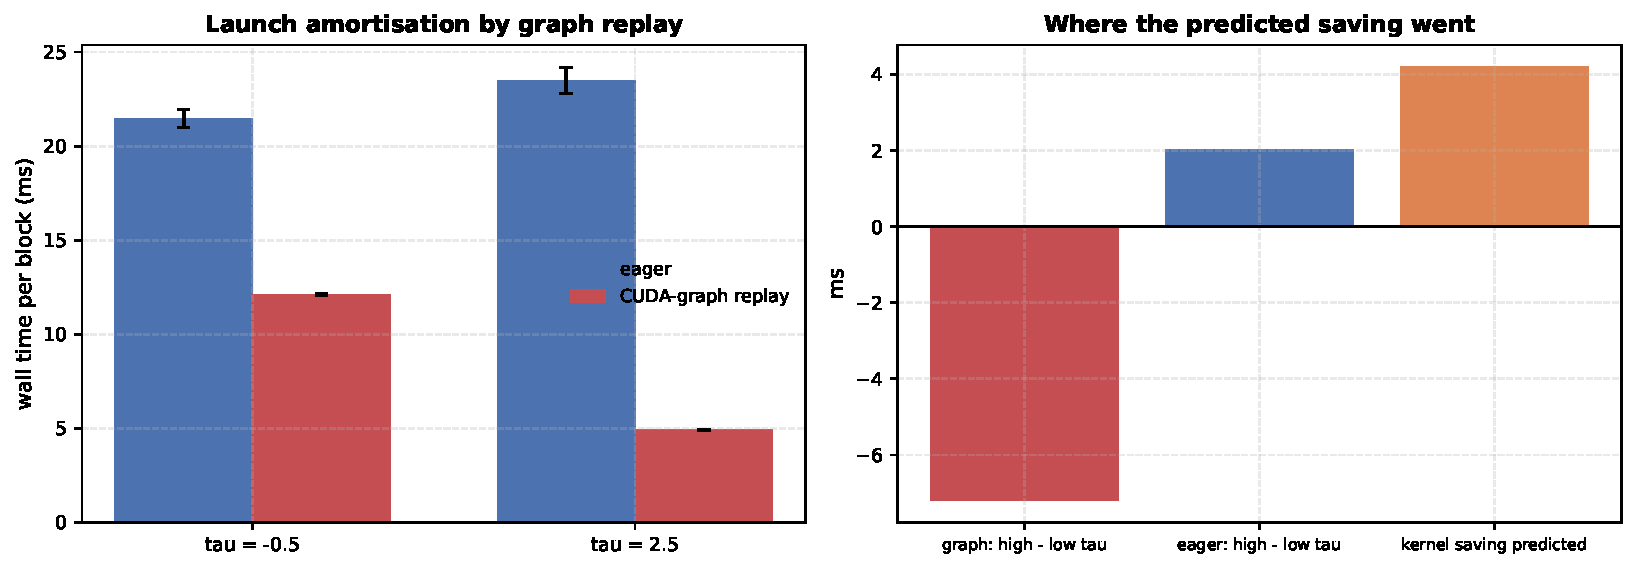
\includegraphics[width=0.98\textwidth]{figures/fig11_cuda_graph_launch_amortization.pdf}
\caption{Launch amortisation isolated by CUDA-graph replay. Left: wall time per block of the 6-layer stack under eager execution and under graph replay, for two thresholds; error bars are the standard error over the measured blocks of a single run. Right: the high-minus-low threshold difference under graph replay and under eager execution, against the saving predicted from the kernel measurement. Source: \texttt{results/exp4c\_cuda\_graphs.json} (\texttt{combined}, \texttt{attribution}).}
\label{fig:11-cuda-graph-launch-amortization}
\end{figure}

\begin{figure}[ht!]
\centering
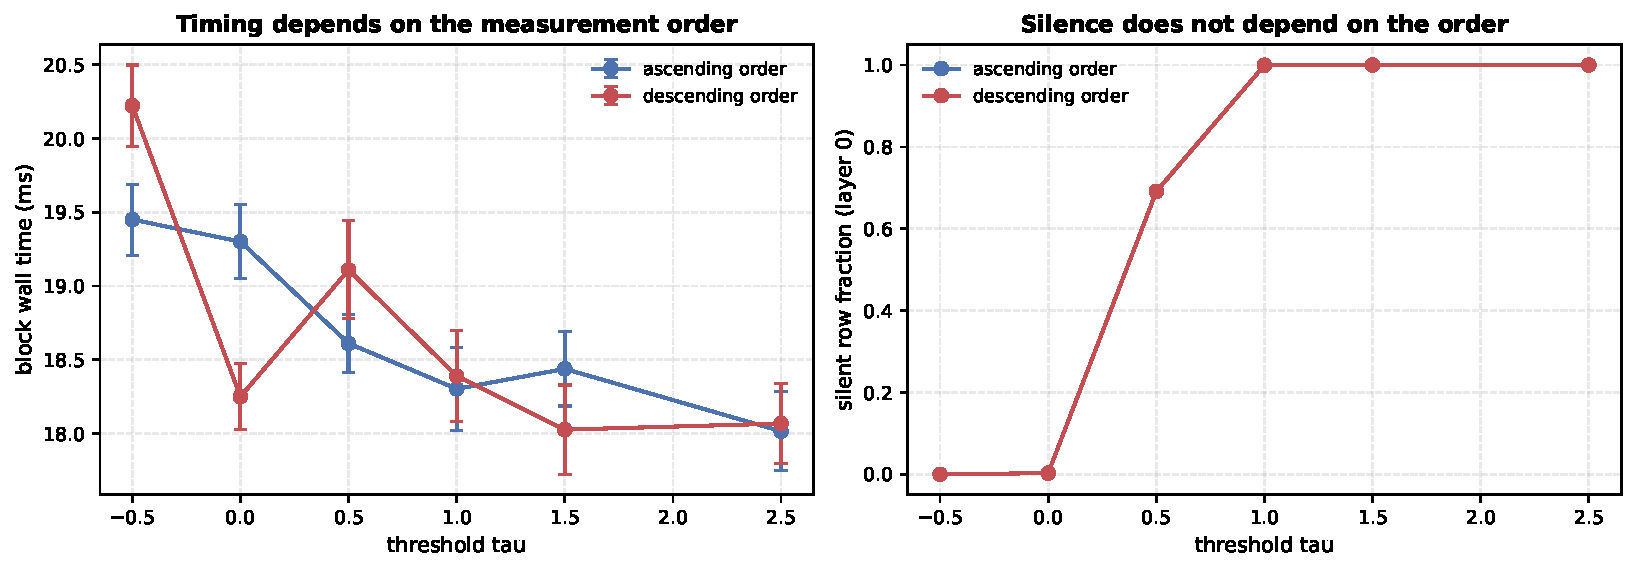
\includegraphics[width=0.98\textwidth]{figures/fig14_measurement_order_drift.pdf}
\caption{Sensitivity of the block timing to the order in which the thresholds are measured. Left: block wall time against threshold, one line per measurement order; error bars are the standard error over the blocks of a single run. Right: the silent-row fraction of the first layer, which does not depend on the order. Source: \texttt{results/exp4b\_sequential\_repro.json} (\texttt{runs}).}
\label{fig:14-measurement-order-drift}
\end{figure}

\begin{figure}[ht!]
\centering
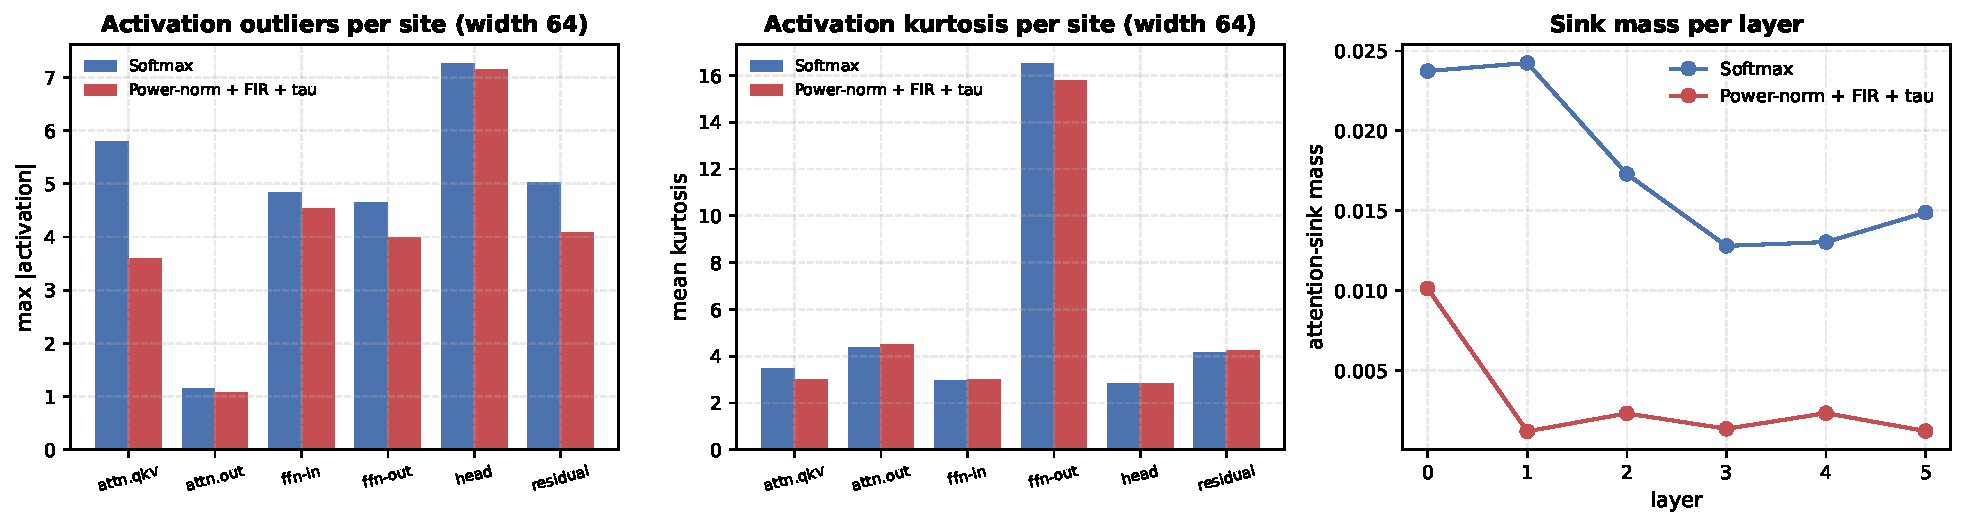
\includegraphics[width=0.98\textwidth]{figures/fig12_int8_outlier_sites.pdf}
\caption{Activation outliers and attention-sink mass of the width-64 runs. Left: maximum absolute activation per site. Middle: mean kurtosis per site. Right: sink mass per layer. One trained checkpoint per variant (no seed spread available). Source: \texttt{results/exp4h\_int8\_quant.json} (\texttt{runs.<run\_id>.outliers}, \texttt{runs.<run\_id>.sink}).}
\label{fig:12-int8-outlier-sites}
\end{figure}

\begin{figure}[ht!]
\centering
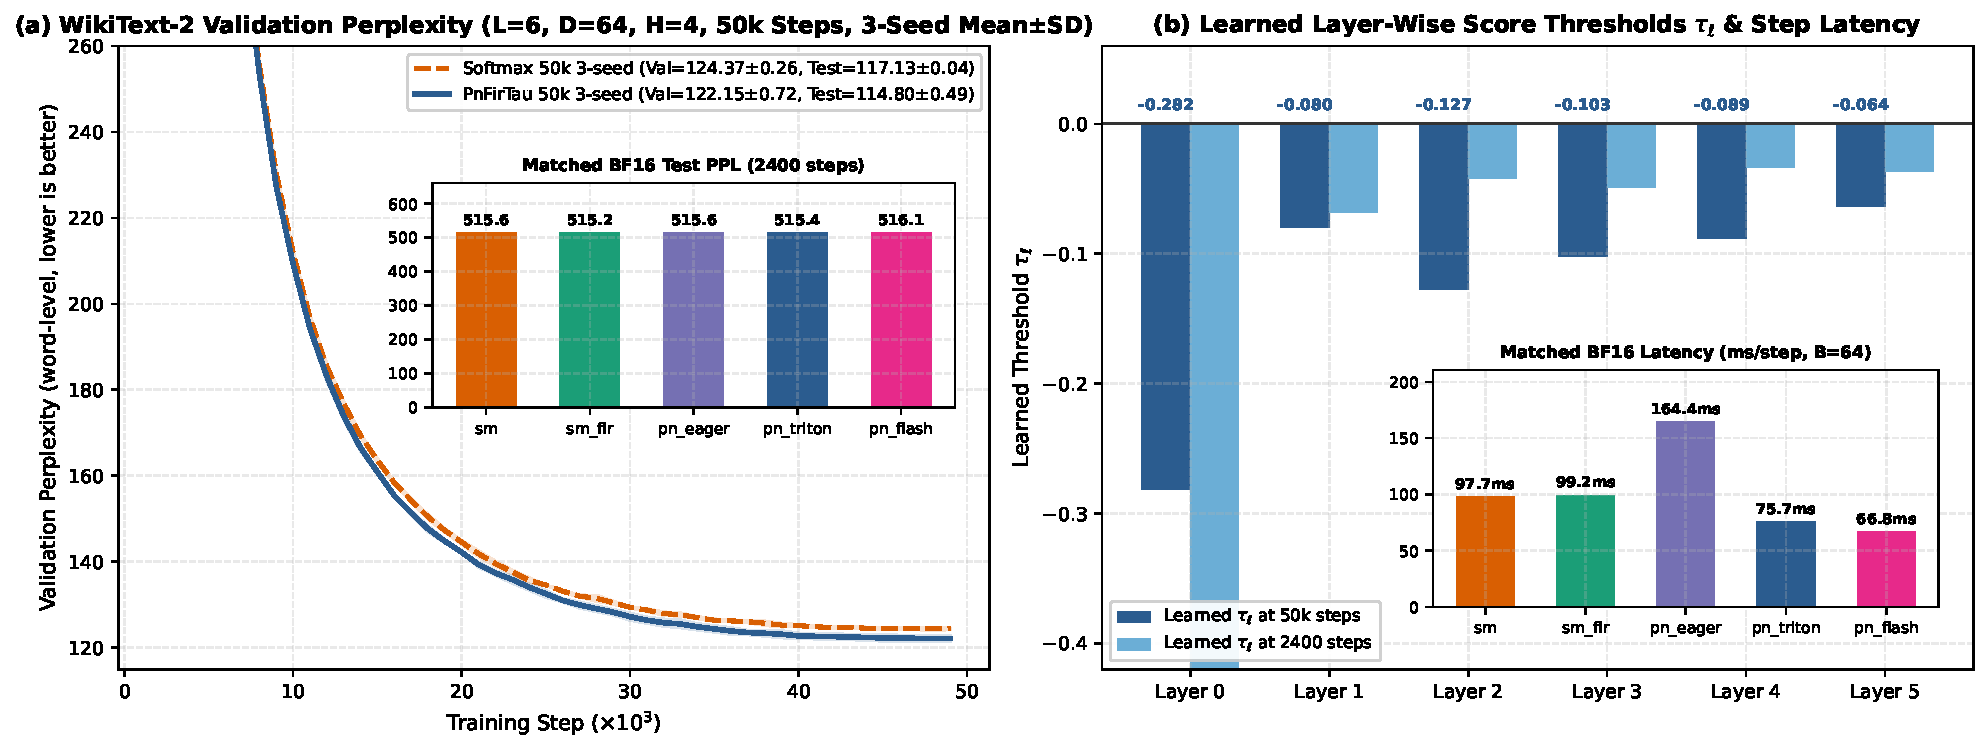
\includegraphics[width=0.98\textwidth]{figures/fig4_wikitext2_lm_and_tau.pdf}
\caption{WikiText-2 50,000-step validation perplexity trajectory (3-seed mean$\pm$SD bands, suite 3 finals in legend) and 2,400-step matched BF16 inset (left), and learned layer-wise thresholds $\tau_\ell$ with matched BF16 step-time inset across all 5 variants (right). Source: \texttt{results/exp4\_wikitext2\_lm.json}, \texttt{results/exp4d\_softmax\_50k\_bf16.json}, \texttt{results/exp4e\_multiseed\_50k.json}.}
\label{fig:wikitext}
\end{figure}

\section{Limitations and Negative Results}
\label{sec:limitations}
Six limitations bound the claims above.
\begin{enumerate}
\item\sloppy \textbf{Scale:} all multi-seed language-modeling results are at $D{=}64$ (1.8M parameters, $L=6$, $\text{seq}{=}256$); a single-seed scale-out at $D{=}256$/$N{=}512$ (10.8M, suite 2s: \texttt{sm\_fir} $359.5$ test, \texttt{pn\_fir\_tau} $377.4$, \texttt{softmax} $379.8$) shows no collapse and preserves the ranking, with a replicated tau profile (layer~0 at $-0.50$). An auxiliary GPT-2 124M retrofit probe (Softmax$\to$\texttt{pn\_fir\_tau} weight transplant, 20k fine-tune steps) reached Test PPL $47.05$ vs.\ $21.43$ for a Softmax retrofit of the same budget; its raw artifacts are not distributed with this work. We attribute the gap to co-adaptation: pre-trained $W_Q,W_K$ are optimized for the translation-invariant geometry of the Softmax simplex, whereas the FIR-induced score shift changes that geometry; a 20k fine-tune cannot re-learn the projection matrices, so the gap is expected. Continuous pre-training or low-rank/evolutionary adaptation is the appropriate protocol at this scale; no GPT-2-class result is claimed. At 1.8M parameters attention sinks are present but modest (Exp 4h: max position-0 mass 1.9\%), so sink-suppression benefits are bounded at this scale. RAG-style behavior is evaluated on a controlled synthetic task, not on a production retrieval corpus.
\item \textbf{Matched 50k with variance, small scale:} Table~\ref{tab:exp4} (suite 3) is precision-controlled across 3 seeds per variant, with a $-2.22 \pm 0.46$ val / $-2.33 \pm 0.49$ test PPL gap for \texttt{pn\_fir\_tau}, holding on all 3 seeds; pn shows larger seed spread than softmax (val std $0.72$ vs.\ $0.26$), and all results are at $D{=}64$ with no larger-model replication. All quoted throughput numbers are single-seed.
\item \textbf{Tile-granularity and launch serialisation:} silent-tile skipping accelerates the isolated kernel ($1.48\times$ re-measured, $1.76\times$ original) but is launch-serialised in the 6-layer stack ($\approx$372 CUDA launches per step, invariant across $\tau$ and $B \in \{4,16\}$; wall unchanged at $4\times$ less GPU work under WSL2 GPU-PV). The end-to-end stack saving attributed to tile skipping (\ref{tab:exp4_skip}, \texttt{mha6} column) was reproduced and falsified as a block-order artifact by the drift-controlled re-measurement (\texttt{exp4b}). A CUDA-graph replay confirms the mechanism by intervention: amortising launches surfaces the saving fully ($12.10 \pm 0.03 \to 4.91 \pm 0.02$ ms, $\Delta = -7.20 \pm 0.02$ ms, \texttt{exp4c}).
\item \textbf{Decoy flooding is memory-length-specific:} exact copies of the queried key at high multiplicity ($n_d \ge 4$; $56.9\%$ at $n_d{=}8$, $\epsilon{=}0.2$ under the 7-tap FIR) do not defeat short-memory linear filtering: a 2-tap shift holds $99.9\% \pm 0.2\%$ (\texttt{sm\_shiftmu}) and $92.7\% \pm 10.4\%$ (\texttt{pn\_shiftmu\_tau}) at $n_d{=}8$ (Exp~6), so the failure is specific to the 7-tap memory length, at the cost of seed-dependent $\tau$--$\mu$ equilibria in the rectified branch.
\item \textbf{$\tau$ calibration regime:} under positive-only training, gradients on $\tau$ come from active rows only, so its resting point against pure-noise rows varies across seeds unless the post-warmup absent-key penalty (\texttt{pn\_fir\_tau\_reg}) is applied.
\item \textbf{Hyperparameter sensitivity:} $p=10$ and $\sigma=2.0$ are fixed a priori; a sensitivity sweep over these values is left for future work.
\end{enumerate}

\section{Conclusion and Practical Guide for Transformer Designers}

We have shown that causal FIR temporal smoothing strictly on $K$ enables single-layer content-addressable value-slot binding ($W_{\text{query}, j^*+1} = 0.729\text{--}0.792$, lifting clean recall from $35.8\%\text{--}44.5\%$ to $100.0\% \pm 0.0\%$ on Exp~1 and Exp~2), established mass constancy along uniform shift rays (Proposition~\ref{thm:dilemma}), explained why uncalibrated \texttt{pn\_fir} suffers score-shift starvation on positive-only training while simplex normalizers (\texttt{Softmax}, \texttt{Sparsemax}, \texttt{Entmax}) fail residual preservation on unanswerable queries ($27.2\%\text{--}34.4\%$ hallucination rate in Exp~5) and row-mean centering (\texttt{pn\_fir\_c}) leaks $\approx 124\times$ more noise ($\sum W_{\text{unans}} = 0.265$), and demonstrated that \texttt{pn\_fir\_tau} achieves $100.0\% \pm 0.0\%$ residual preservation ($0.0\%$ hallucination rate, $\sum W_{\text{unans}} = 0.002 \pm 0.002$, $50\times$ lower continuous residual leakage than \texttt{Softmax\_1} and \texttt{Quiet Softmax}) under pure Cross-Entropy loss while matching and slightly improving 6-layer WikiText-2 perplexity at 1.8M parameters.

For practitioners building and deploying Transformer models, our findings translate into two actionable architectural takeaways:
\begin{enumerate}
\item \textbf{Immediate Zero-Parameter Single-Layer Induction (\texttt{sm\_fir}):} If the primary goal is to equip a standard causal Transformer with single-layer key-value induction binding (compressing two-layer induction heads into one layer) without custom attention kernels, applying the fixed 7-tap causal Gaussian FIR filter strictly to the key tensor $K$ (\texttt{sm\_fir}) requires zero learnable parameters, adds only $+1.5\%$ step-time overhead in \texttt{BF16} ($+2.0\%$ in \texttt{FP32}), and can be paired with \texttt{triton\_causal\_fir} for zero-copy strided filtering.
\item\sloppy \textbf{Hallucination-Free Residual Preservation, Sink-Free Attention, and Transcendental-Free Hardware Acceleration (\texttt{pn\_fir\_tau\_triton} / \texttt{pn\_fir\_tau\_flash}):} If the architecture requires attention heads to \textbf{abstain cleanly when queried information is absent from the context}---such as RAG over noisy passages, memory-augmented Transformers, or models designed for low-bit INT4/INT8 quantization and streaming KV caches without \texttt{BOS} Attention-Sink outliers---replacing simplex normalizers with sub-simplex rectified power-normalization (\texttt{pn\_fir\_tau}) eliminates context-induced residual hallucinations ($0.0\%$ vs.\ $27.2\%\text{--}34.4\%$ for \texttt{Softmax}/\texttt{Sparsemax}/\texttt{Entmax}) and suppresses continuous absent-key residual leakage $50\times$ more tightly than virtual-sink Softmax. Moreover, when deployed via our fused Triton kernels (\texttt{PnFirTauTritonMHA} and \texttt{PnFirTauFlashMHA} in \texttt{src/triton\_pnfirtau.py}), evaluating $(S'_{t,j})_+^{10}$ in 3 register multiplications with zero \texttt{exp()} calls and zero online tile rescaling reduces full-LM \texttt{BF16} step time by \textbf{$22.5\%\text{--}31.6\%$ below standard \texttt{Softmax}} ($2.17\times\text{--}2.46\times$ faster than eager PyTorch) and achieves \textbf{$21.70\times$ speedup ($6.97\times$ vs.\ \texttt{softmax}) and $66.5\times$ VRAM reduction} on a 6-layer MHA stack at $N=1024, B=16$.
\end{enumerate}

\section*{Declarations}

\paragraph{Competing interests.} The author declares no competing interests.

\paragraph{Funding.} This research received no external funding.

\paragraph{Data and code availability.} The reproducibility package (source code, experiment suites, raw JSON results, and figure-generation pipeline) is provided with this preprint; an archived copy will be deposited on Zenodo upon publication.

\paragraph{Author contributions.} M.Z. conceived the study, implemented the method and kernels, ran the experiments, analysed the results, and wrote the manuscript.

\paragraph{Ethics.} Not applicable; this study uses no human or animal subjects.

\begin{thebibliography}{15}
\bibitem{zhang2021rela}
B.~Zhang, I.~Titov, and R.~Sennrich, ``Sparse attention with linear units,''
\emph{arXiv:2104.07012}, 2021.

\bibitem{zuhri2025softpick}
Z.~M.~K. Zuhri, E.~H.~Fuadi, and A.~F.~Aji, ``Softpick: No attention sink, no massive
activations with rectified softmax,'' \emph{arXiv:2504.20966}, 2025.

\bibitem{wang2026abstention}
R.~Z.~Wang, ``Abstention and noise filtering: Two missing primitives of softmax attention,''
\emph{arXiv:2609.22005}, 2026.

\bibitem{sun2024massive}
M.~Sun, X.~Chen, J.~Z.~Kolter, and Z.~Liu, ``Massive activations in large language models,''
\emph{arXiv:2402.17762}, 2024.

\bibitem{peng2023rwkv}
B.~Peng, E.~Alcaide, Q.~Anthony, et~al., ``RWKV: Reinventing RNNs for the transformer era,''
in \emph{Findings of the Association for Computational Linguistics: EMNLP 2023}, 2023,
pp.~14048--14077, doi:10.18653/v1/2023.findings-emnlp.936 (preprint: \emph{arXiv:2305.13048}).

\bibitem{olsson2022induction}
C.~Olsson, N.~Elhage, N.~Nanda, et~al., ``In-context learning and induction heads,''
\emph{Transformer Circuits Thread}, 2022, \emph{arXiv:2209.11895}.

\bibitem{vaswani2017attention}
A.~Vaswani, N.~Shazeer, N.~Parmar, et~al., ``Attention is all you need,'' in
\emph{Advances in Neural Information Processing Systems (NeurIPS)}, vol.~30, 2017,
\emph{arXiv:1706.03762}.

\bibitem{so2021primer}
D.~R.~So, W.~Ma\'{n}ke, H.~Liu, Z.~Dai, N.~Shazeer, and Q.~V.~Le, ``Primer: Searching for
efficient transformers for language modeling,'' in \emph{Advances in Neural Information
Processing Systems (NeurIPS)}, vol.~34, 2021, \emph{arXiv:2109.08668}.

\bibitem{martins2016sparsemax}
A.~F.~T.~Martins and R.~F.~Astudillo, ``From softmax to sparsemax: A sparse model of attention
and multi-label classification,'' in \emph{International Conference on Machine Learning (ICML)},
2016, \emph{arXiv:1602.02068}.

\bibitem{peters2019sparse}
B.~Peters, V.~Niculae, and A.~F.~T.~Martins, ``Sparse sequence-to-sequence models,'' in
\emph{Annual Meeting of the Association for Computational Linguistics (ACL)}, 2019,
pp.~1504--1519, doi:10.18653/v1/P19-1146 (preprint: \emph{arXiv:1905.05702}).

\bibitem{correia2019adaptively}
G.~M.~Correia, V.~Niculae, and A.~F.~T.~Martins, ``Adaptively sparse transformers,'' in
\emph{Conference on Empirical Methods in Natural Language Processing and the 9th International
Joint Conference on Natural Language Processing (EMNLP-IJCNLP)}, 2019, pp.~2174--2184,
doi:10.18653/v1/D19-1223 (preprint: \emph{arXiv:1909.00015}).

\bibitem{miller2023offbyone}
E.~Miller, ``Attention is off by one,'' online post, July 24, 2023.
[Online]. Available: \url{https://www.evanmiller.org/attention-is-off-by-one.html}.
[Accessed: October 19, 2026].

\bibitem{bondarenko2023quantizable}
Y.~Bondarenko, M.~Nagel, and T.~Blankevoort, ``Quantizable transformers: Removing outliers by
helping attention heads do nothing,'' in \emph{Advances in Neural Information Processing
Systems (NeurIPS)}, vol.~36, 2023, \emph{arXiv:2306.12929}.

\bibitem{xiao2024streamingllm}
G.~Xiao, Y.~Tian, B.~Chen, S.~Han, and M.~Lewis, ``Efficient streaming language models with
attention sinks,'' in \emph{International Conference on Learning Representations (ICLR)}, 2024,
\emph{arXiv:2309.17453}.

\bibitem{dao2022flashattention}
T.~Dao, D.~Y.~Fu, S.~Ermon, A.~Rudra, and C.~R\'{e}, ``FlashAttention: Fast and memory-efficient
exact attention with IO-awareness,'' in \emph{Advances in Neural Information Processing
Systems (NeurIPS)}, vol.~35, 2022, \emph{arXiv:2205.14135}.
\end{thebibliography}

\end{document}
